% =============================================================
%  tinyCPG paper — main LaTeX file
%
%  Compile with:  latexmk -pdf main.tex
%  (or)           pdflatex main && bibtex main && pdflatex main && pdflatex main
%
%  Generic preamble suitable for either PLOS Computational Biology
%  or Frontiers in Computational Neuroscience. Switch to the
%  publisher's template at submission time by replacing the
%  `\documentclass` and `\bibliographystyle` lines.
% =============================================================

\documentclass[11pt,letterpaper]{article}

\usepackage[utf8]{inputenc}
\usepackage[T1]{fontenc}
\usepackage{lmodern}
\usepackage[margin=1in]{geometry}
\usepackage{amsmath, amssymb}
\usepackage{graphicx}
\graphicspath{{figures/}}
\usepackage{xcolor}
\usepackage{hyperref}
\hypersetup{colorlinks=true, linkcolor=blue!50!black,
            citecolor=blue!50!black, urlcolor=blue!70!black}
\usepackage{booktabs}
\usepackage{caption}
\captionsetup{font=small, labelfont=bf, format=plain}
\usepackage{siunitx}        % for SI units in tables
\usepackage{enumitem}
\setlist{nosep}

% TODO / margin-note macros to make scaffold work visible
\newcommand{\todo}[1]{\textcolor{red}{\textbf{[TODO: #1]}}}
\newcommand{\xref}[1]{\textcolor{purple}{[\textsc{#1}]}}  % cross-ref placeholders

\title{Self-organisation of a closed-loop spinal locomotor pattern: \\
       extending the Rybak-style central pattern generator with STDP,
       motoneurons, and Ia sensory feedback}

\author{Maxim Talanov\textsuperscript{1,*} \\
        \textit{\small \textsuperscript{1}Affiliation (TODO)} \\
        \textit{\small \textsuperscript{*}Correspondence: max.talanov@gmail.com}}

\date{}

% =============================================================
\begin{document}
\maketitle

% Abstract — target 200-250 words for PLOS Comp Bio, up to 350 for Frontiers
% in Comp Neuro. Numbers from results/2026-09-25_ftgrid and round 6.

\begin{abstract}
\noindent
Computational models of the spinal central pattern generator (CPG) in the
Rybak/Danner/Zhang lineage capture interlimb coordination in detail but, by
their authors' own account, omit motoneurons, muscle dynamics, sensory
feedback and synaptic plasticity, and prescribe every synaptic weight by
hand. We asked whether a spinal CPG closed in a loop with its periphery can
tune its own synapses to a working gait. We built a two-leg spiking model of
the rat lumbar CPG in NEST: Izhikevich rhythm-generator half-centres with
asymmetric reciprocal inhibition, motoneuron pools driving muscle proxies with
force, length and fatigue, Ia feedback into the reciprocal-inhibition core, and
spike-timing-dependent plasticity (STDP) on the cutaneous and brainstem inputs
to the rhythm generators. Stance is not ended by a clock: each leg's stance
ends when its own extensor force falls. From ten initial weight distributions
($0$--$16$\,pA) the plastic synapses converge to the same values (cutaneous
$\approx61$\,pA, brainstem $\approx16$\,pA) and produce the same alternating
gait. Across four locomotion modes --- slow, medium and fast walk, and toe
stepping under partial unloading --- and five learning rates, learning that
converges within the session yields force-triggered, alternating stepping in
every mode (extensor--flexor force correlation $-0.47$ to $-0.75$;
left--right $-0.32$ to $-0.81$). Without learning the rhythm falls back on a
safety timer, and a partially learned synapse produces the least coordinated
gait of all. Partial unloading slows learning without abolishing the gait.
The sensorimotor gains of a spinal CPG can thus be learned rather than
prescribed, and whether the closed loop takes over depends on how much
plasticity is available --- a mechanistic account relevant to activity-based
rehabilitation after incomplete spinal cord injury.
\end{abstract}

\noindent\textbf{Keywords:} spinal central pattern generator, STDP,
locomotion, sensory feedback, force-triggered stepping, spinal cord injury,
rehabilitation, NEST simulator.


\section{Introduction}\label{sec:intro}
% Introduction — target 600-900 words for PLOS Comp Bio.
% Funnel: broad CPG context  →  Rybak/Danner/Zhang lineage  →
%        their stated limitations  →  our four extensions  →  paper roadmap.

\todo{4-6 paragraphs. Suggested outline below.}

\paragraph{$\bullet$ Paragraph 1 --- CPG context.}
Coordinated rhythmic limb movement in mammals is controlled primarily by
spinal cord circuitry~\cite{grahamBrown1911,kiehn2006,kiehn2016}.
Rhythm-generating (RG) circuits in the cervical and lumbar enlargements
produce flexor and extensor bursts that drive locomotor output, with the
characteristic flexor--extensor counter-phase pattern preserved across
species. \emph{The remainder of P1: a sentence on why a quantitative
computational understanding matters (e.g.\ for neural prosthetics,
recovery-after-injury models, robotics-of-locomotion).}

\paragraph{$\bullet$ Paragraph 2 --- Rybak/Danner/Zhang model lineage.}
A succession of biophysically detailed computational models has
progressively refined the architecture of the central spinal
CPG~\cite{rybak2006,shevtsova2015,danner2017,zhang2022}. These models use
Hodgkin--Huxley dynamics with persistent-sodium-driven intrinsic bursting,
typed genetic interneuron populations (V0V, V0D, V1, V2a, V3, Shox2), and
hand-curated synaptic weights. The most recent extension~\cite{zhang2022}
adds ascending long-propriospinal V3 neurons to reproduce
speed-dependent gait expression (walk, trot, gallop, bound) in mice.

\paragraph{$\bullet$ Paragraph 3 --- Acknowledged limitations.}
This lineage of models, however, makes three deliberate
simplifications, explicitly listed by~\cite{zhang2022}: (i)
\emph{``the model does not include motoneurons''}; (ii) \emph{``the
model focuses exclusively on central interactions within the spinal cord,
without considering biomechanics and the role of sensory feedback from the
limbs''}; (iii) reflex circuits mediated by Ia and Ib interneurons,
Renshaw cells, and pattern-formation interneurons are absent. In
addition, all synaptic weights in these models are \emph{hand-tuned}; no
form of synaptic plasticity is considered.

\paragraph{$\bullet$ Paragraph 4 --- Our extensions.}
Here we extend this lineage with four mechanisms:
(1) STDP-driven self-organisation of descending (BS$\to$RG) and
cutaneous (CUT$\to$RG) synapses, removing the need to hand-tune
afferent weights;
(2) closed-loop force-driven Ia spindle feedback projecting back into
the reciprocal-inhibition interneurons (InE, InF);
(3) motoneuron pools and Hill-style muscle proxies producing
graded force and length traces;
(4) externally paced sequential Ia activation modelling
heel$\to$mid$\to$toe pressure transfer during the stance phase.

\paragraph{$\bullet$ Paragraph 5 --- Scope and non-scope.}
We deliberately retain the present-paper scope to a two-leg
(left/right hindlimb) system. The four-limb fore--hindlimb
coordination captured by V3 ascending long-propriospinal neurons
in~\cite{zhang2022} is beyond the present scope. We do not attempt
to reproduce gait \emph{transitions} (walk$\to$trot$\to$gallop$\to$bound)
either: the present focus is on stability of a single paced gait under
self-organised weights, across the rat locomotor speed range
(\SIrange{600}{1400}{\milli\second} step period).

\paragraph{$\bullet$ Paragraph 6 --- Paper roadmap.}
Section~\ref{sec:methods} describes the model architecture, Izhikevich
neuron parameters, STDP rule, sensory pathways, and the paced gait
protocol. Section~\ref{sec:results} presents (i) STDP convergence and
long-term stability of the paced locomotor pattern over
\SI{120}{\second}, (ii) an ablation budget identifying which components
are necessary, and (iii) a speed sweep showing that the gait tracks
commanded step period within tens of microseconds across the rat
locomotor range. Section~\ref{sec:discussion} positions the work
relative to the Rybak lineage and discusses limitations and future
extensions.


\section{Methods}\label{sec:methods}
% Methods — see paper/methods_skeleton.md for the long-form outline.
% Target 1500-2000 words for PLOS Comp Bio. Each subsection below maps to
% a markdown subsection in methods_skeleton.md.

\subsection{Model overview}\label{sec:methods:overview}
The two-leg spinal CPG presented here extends a canonical computational
sCPG model~\cite{rybak2006,shevtsova2015} with four
mechanisms not present in the Zhang 2022 reference model~\cite{zhang2022}:
(i) STDP-driven self-organisation of descending and cutaneous afferent
synapses onto the rhythm generator;
(ii) a closed-loop Ia feedback pathway to the reciprocal-inhibition
interneurons;
(iii) motoneuron pools driving Hill-like muscle proxies with force and
length dynamics;
(iv) closed-loop, force-triggered stance/swing switching: each leg's
cutaneous (paw-contact) input is switched on and off by that leg's own
extensor force rather than by a clock, with sequential Ia activation
simulating heel-to-toe weight transfer within each stance.
The model is implemented in NEST~3.9~\cite{nest2002} and is publicly
available at \href{https://github.com/max-talanov/tinyCPG}{github.com/max-talanov/tinyCPG}.

\begin{figure}[t]
  \centering
  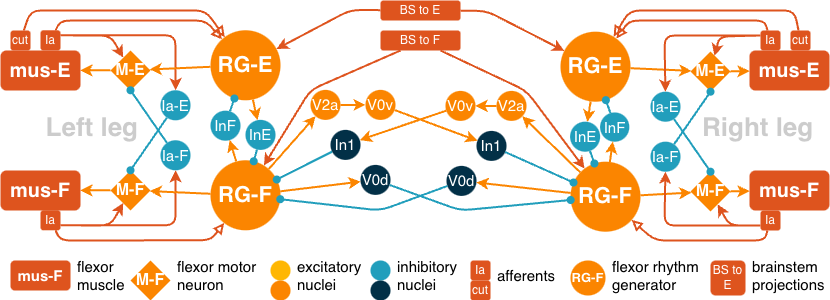
\includegraphics[width=0.8\textwidth]{fig1_schematic.png}
  \caption{\textbf{Architecture of the two-leg spinal CPG.}
    Each leg contains a flexor (F)
    and extensor (E) rhythm-generator half-centre coupled by asymmetric
    reciprocal inhibition via InE and InF interneurons (Zhang 2022 6:1
    ratio). Sensory afferents (Ia, cutaneous) feed into the
    reciprocal-inhibition interneurons; motor pools (M-E, M-F) drive
    muscle proxies whose force and length signals close the Ia loop.
    L\,$\leftrightarrow$\,R commissural inhibition (V0-like) is mediated by
    flexor- and extensor-targeted projections.}
  \label{fig:schematic}
\end{figure}

\subsection{Single-neuron model}\label{sec:methods:neuron}
The network is implemented at two complementary levels of biophysical
detail, using the same architecture, the same plastic projections and the
same experimental protocol in both cases.

\paragraph{Reduced (Izhikevich) implementation.}
In the NEST implementation, all spiking neurons are modelled as Izhikevich
quadratic-integrate-fire units~\cite{izhikevich2003}. Each neuron obeys
\begin{align}
  \frac{dv}{dt} &= 0.04v^2 + 5v + 140 - u + I, \\
  \frac{du}{dt} &= a\,(bv - u),
\end{align}
with the after-spike reset $v \leftarrow c$, $u \leftarrow u + d$ applied
whenever $v \geq 30$\,mV. Excitatory extensor RG-E neurons use the
regular-spiking set ($a=0.02, b=0.2, c=-65, d=8$). Flexor RG-F neurons use
the intrinsically-bursting set ($a=0.02, b=0.2, c=-55, d=4$), which
approximates persistent-sodium-driven ($I_\text{NaP}$) bursting
phenomenologically rather than deriving it from channel kinetics.
Inhibitory interneurons (InE, InF, Ia-INT) use a fast-spiking set
($d=2$). This formulation reproduces the spiking and bursting regimes
required by the rhythm generator at a small fraction of the computational
cost of a conductance-based model, which is what makes the large
mode\,$\times$\,learning-rate parameter sweeps reported here tractable.

\paragraph{Conductance-based (Hodgkin--Huxley) implementation.}
Because the reduced model represents bursting phenomenologically, we also
implemented the same circuit with conductance-based neurons in
NEURON~\cite{hines1997}, following the Hodgkin--Huxley
formalism~\cite{hodgkinHuxley1952}. Membrane potential evolves as
\begin{equation}
  C_m \frac{dV}{dt} = -\!\sum_i g_i\, m_i^{p}h_i^{q}\,(V - E_i) - I_\text{leak} + I_\text{syn},
  \label{eq:hh}
\end{equation}
where each active conductance $g_i$ is gated by activation ($m_i$) and
inactivation ($h_i$) variables obeying first-order kinetics
$\dot{x} = (x_\infty(V) - x)/\tau_x(V)$. Rhythm-generator neurons include
fast sodium, delayed-rectifier potassium and leak conductances together
with an explicit persistent sodium current ($I_\text{NaP}$), so that
bursting arises from channel kinetics rather than from a reset rule.
Motoneurons and interneurons are multi-compartment cells with somatic and
dendritic sections. This implementation resolves the sub-threshold and
channel-level dynamics that the Izhikevich formulation abstracts away, at
substantially higher computational cost; it therefore serves as a
biophysical cross-check on the reduced model rather than as the vehicle
for the full parameter sweep.%
\todo{The NEURON/HH results are not yet included in Results. Until they
are, this subsection describes an implementation the paper does not yet
report on, and the Limitations no longer flag the absence of a
conductance-based model --- add the HH results (or re-scope this
paragraph) before circulating.}

Synaptic delays in both implementations are drawn from a rat
\texttt{length\_velocity} preset (Table~\ref{tab:delays}) with
$\sigma=0.2$\,ms Gaussian jitter.

\subsection{Network architecture}\label{sec:methods:network}

\paragraph{Asymmetric reciprocal inhibition (Zhang 2022).}
The F$\to$InF$\to$E pathway is strong ($W_{\text{InF}\to\text{RG-E}}=-48$\,pA,
$P=0.30$); the E$\to$InE$\to$F pathway is weak
($W_{\text{InE}\to\text{RG-F}}=-8$\,pA, $P=0.15$).
The 6:1 ratio preserves the flexor's role as the rhythm-leading
half-centre~\cite{zhang2022,talpalar2013}.

\paragraph{Closed-loop Ia$\to$reciprocal-IN pathway (this work).}
Ia-E parrots project to InE ($W=6$\,pA, $P=0.25$) and Ia-F parrots to
InF, providing closed-loop sensory drive into the reciprocal-inhibition
core. This pathway compensates the loss of strong tonic descending drive
characteristic of deafferented fictive locomotion~\cite{pearson1995,
rossignol2006,hultborn2006}.

\paragraph{Cutaneous reflex.}
Cutaneous parrots project to RG-E (STDP-plastic) and to InE
($W=6$\,pA, $P=0.30$), implementing the stance-phase cutaneous-reflex
gating of extensor activity~\cite{forssberg1980,pearson1995}.

\paragraph{Commissural inhibition.}
L$\leftrightarrow$R flexor RG inhibition is strong
($W=-20$\,pA, $P=0.22$); extensor inhibition is weak
($W=-8$\,pA, $P=0.10$). This V0-mediated commissural inhibition
enforces left--right alternation~\cite{kiehn2016,talpalar2013}.

\paragraph{Motor pool, muscle relay.}
Each motor neuron projects to $N_{\text{mus}}=100$ muscle-parrot relays
($P_{\text{M}\to\text{mus}}=0.8$). Motor pool reciprocal inhibition
($W=-22$\,pA, $P=0.25$) enforces antagonist suppression at the motor
level~\cite{mccreaRybak2008}.

\paragraph{Connectivity specification.}
The full per-connection weight and delay distributions of every
projection were obtained by querying NEST directly after network
construction. Table~\ref{tab:delays}
lists all projections grouped by the functional blocks of the
architecture (Fig.~\ref{fig:schematic}): descending/supraspinal drive,
the sensory afferent$\to$RG projections, the rhythm-generator reciprocal
core, the Ia proprioceptive interneuron pathway, motor output, and the
commissural (interlimb) projections. Static projections are
heterogeneous: their per-connection weights are drawn from a lognormal
distribution about the design value (coefficient of variation $0.5$, mean
and sign preserved), since biological synaptic weights are lognormally
distributed rather than uniform~\cite{song2005,buzsaki2014}. The mean
preserves the designed balance---in particular the asymmetric reciprocal
inhibition (InF$\to$RG-E $=-48$\,pA, InE$\to$RG-F $=-8$\,pA) reproduces the
Zhang~6:1 ratio exactly. The plastic projections (CUT$\to$RG-E and
BS$\to$RG-\{E,F\}) start from a lognormal distribution and are reported
both as initialised and after learning (Fig.~\ref{fig:connectivity}a,b;
Table~\ref{tab:delays}). The cutaneous input to RG-E is a single plastic projection. Conduction delays follow the rat
\texttt{length\_velocity} preset (brainstem pathways $\approx 3.0$\,ms,
reciprocal and motor pathways $\approx 1.8$\,ms, commissural
$\approx 2.2$\,ms) with $0.2$\,ms across-connection jitter. The
muscle$\to$Ia spindle/GTO feedback is implemented as a rate-coded
transduction (force and length $\to$ Ia firing rate), not a synaptic
projection, and so has no weight/delay entry.
Figure~\ref{fig:connectivity} shows the weight and delay distributions.


\begin{figure}[t]
  \centering
  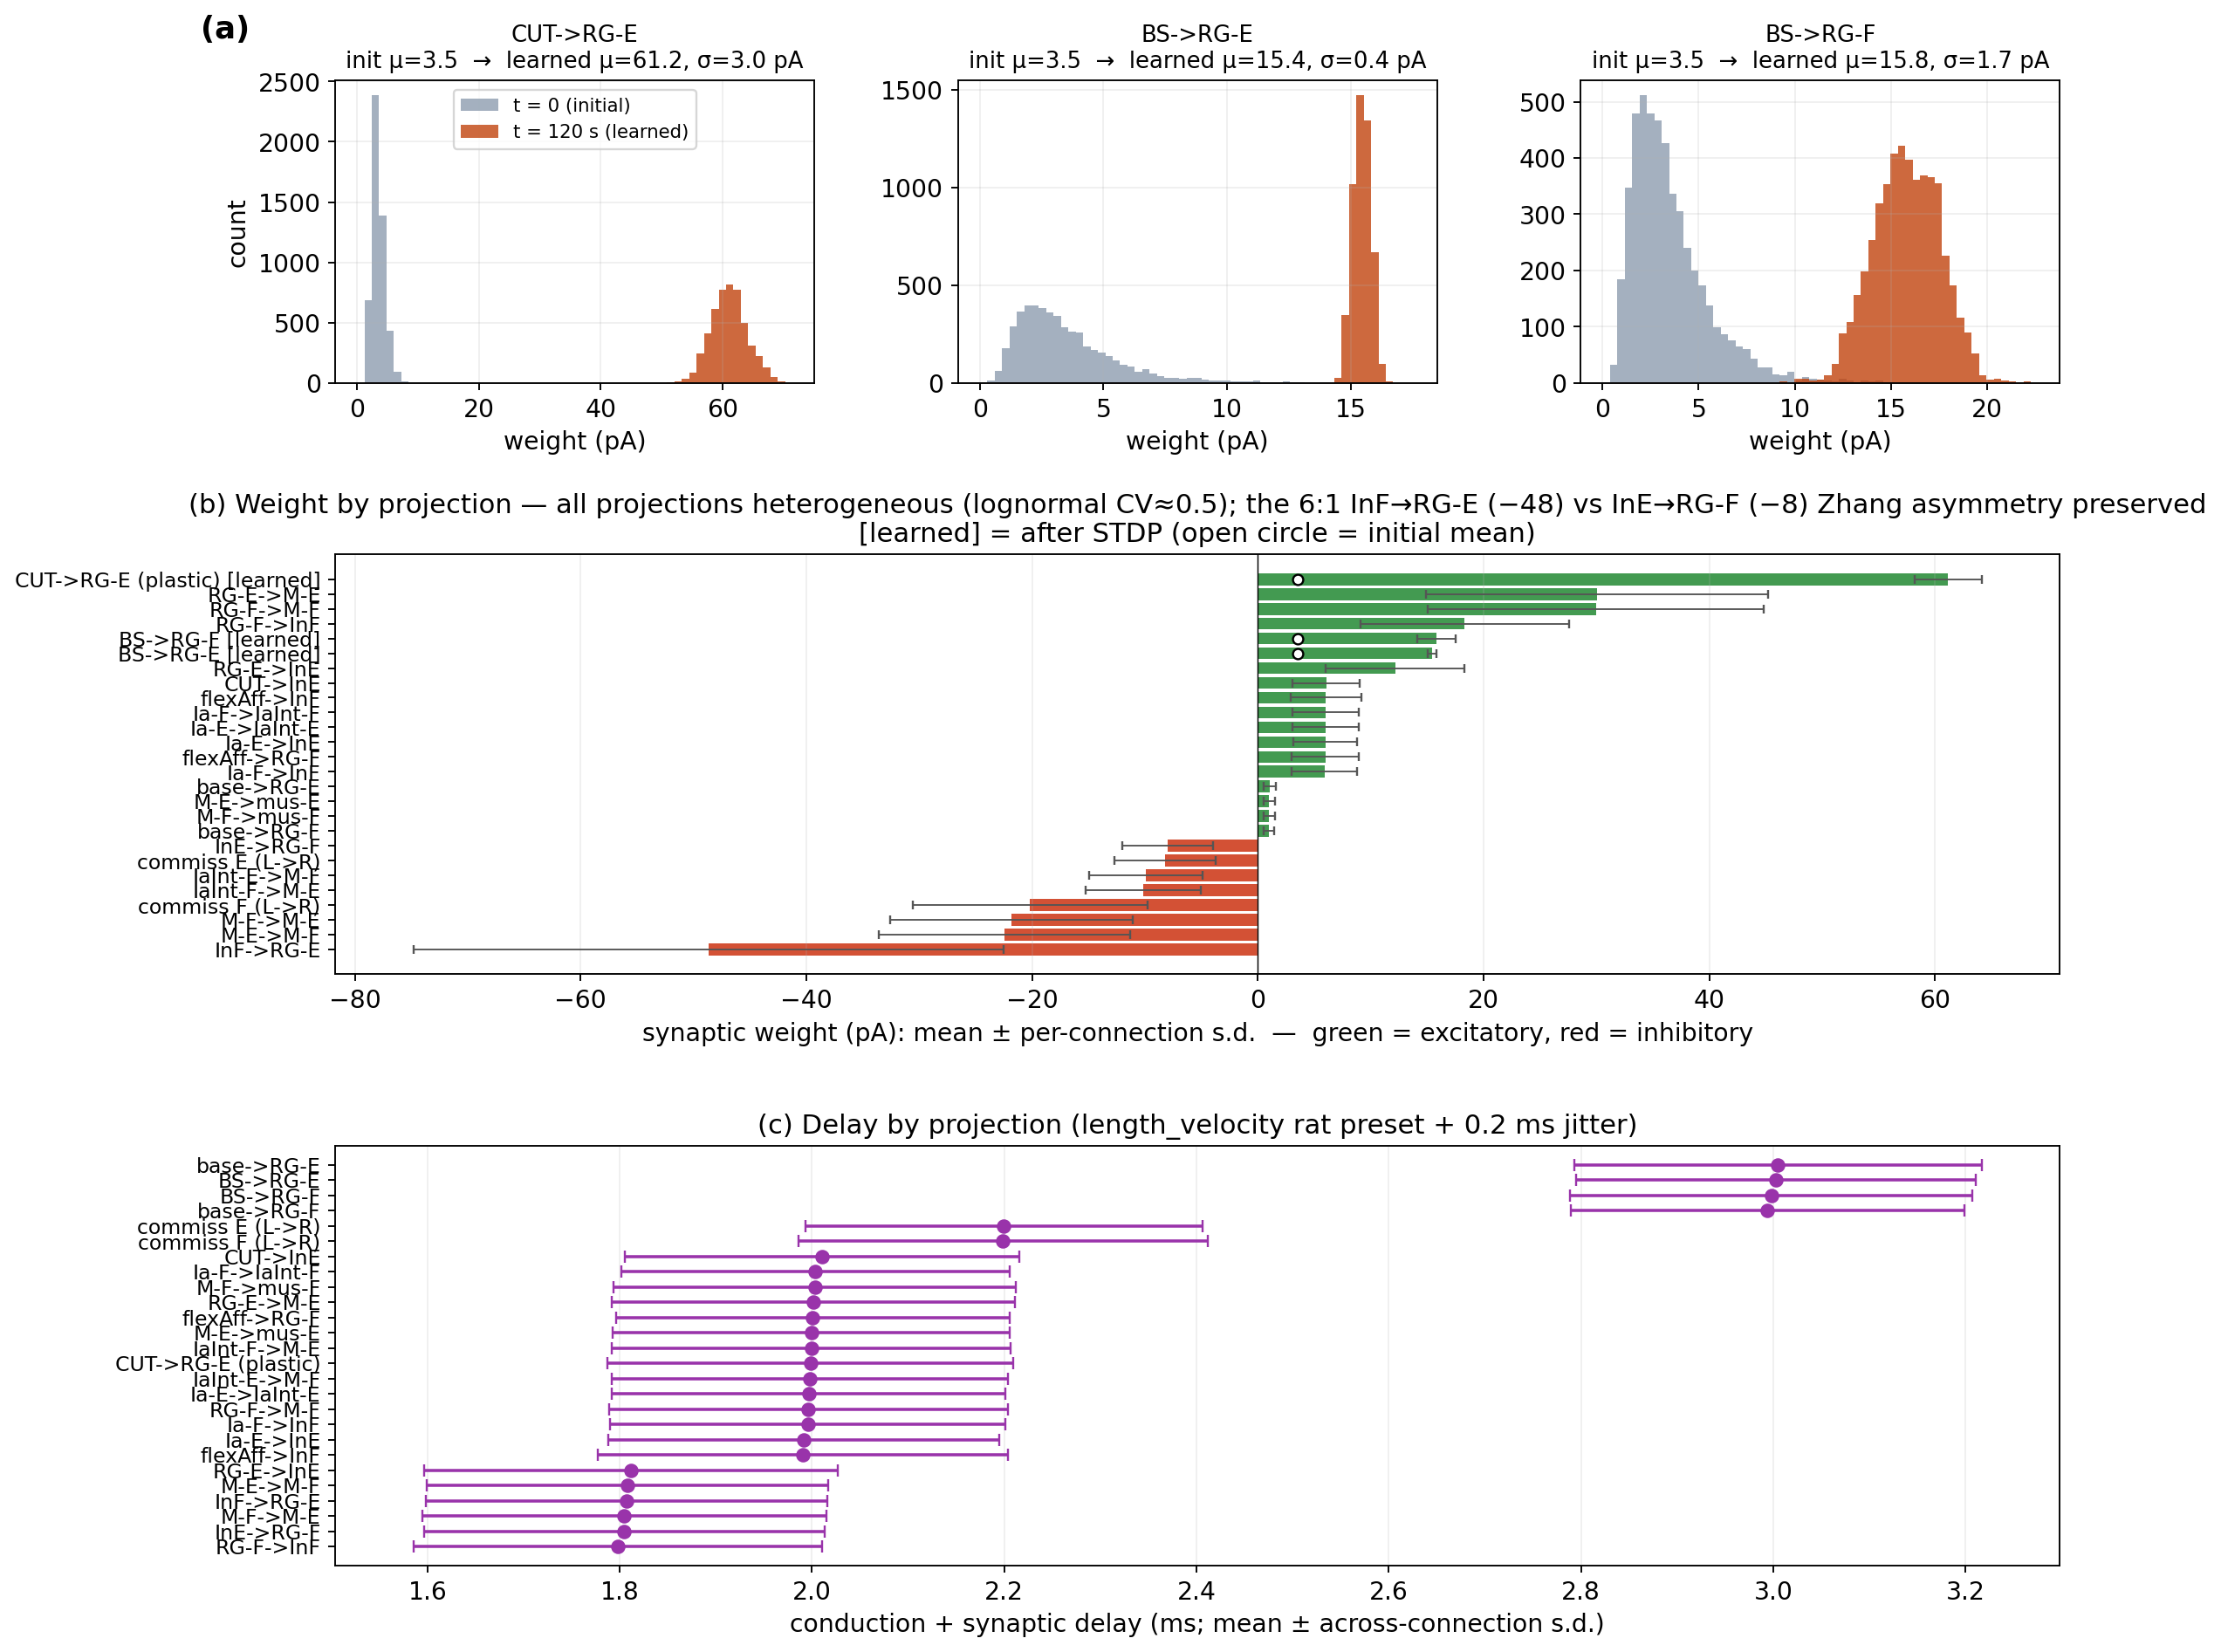
\includegraphics[width=0.8\textwidth]{fig_connectivity.png}
  \caption{\textbf{Synaptic weights and conduction delays along every
  projection, before and after learning.} \textbf{(a)} Weight histograms of
  the three plastic projections, leg L: as initialised (grey, lognormal
  $\mu=3.5$\,pA, CV$=0.3$) and after 120\,s of learning (orange; medium walk,
  $\lambda=10^{-3}$). \textbf{(b)} Synaptic weight per projection (mean $\pm$
  per-connection s.d.; green excitatory, red inhibitory); plastic
  projections are shown at their learned values (open circle = initial
  mean). All static projections are heterogeneous (lognormal, CV$\approx
  0.5$), with the asymmetric reciprocal inhibition InF$\to$RG-E $=-48$\,pA
  versus InE$\to$RG-F $=-8$\,pA preserving the Zhang~6:1 ratio in the mean.
  \textbf{(c)} Conduction~+~synaptic delay per projection (mean $\pm$
  across-connection s.d.), following the rat \texttt{length\_velocity}
  preset with $0.2$\,ms jitter.}
  \label{fig:connectivity}
\end{figure}

\subsection{Brainstem drive}\label{sec:methods:bs}
Reticulospinal input is modelled as a tonic Poisson process at
$BS_{\text{regular}}=60$\,Hz with $\sigma=0.25$\,Hz noise, identical for
both legs. The 60\,Hz value sits in the
middle of the rat reticulospinal range
(20--80\,Hz)~\cite{drew1986,brocard2010}. In contrast to~\cite{zhang2022},
who vary tonic drive $\alpha$ to vary gait speed, we hold the BS firing
rate tonic and let the stance/swing timing emerge from sensory feedback
(see \autoref{sec:methods:paced}); the \emph{strength} of the BS$\to$RG
synapses is learned (\autoref{sec:methods:stdp}).

\subsection{Spike-timing-dependent plasticity}\label{sec:methods:stdp}
Two projections --- cutaneous CUT$\to$RG-E and brainstem
BS$\to$RG-\{E,F\} --- carry multiplicative STDP synapses (NEST
\verb|stdp_synapse|; $\tau_+=20$\,ms, default $\lambda=10^{-3}$,
$\alpha=0.95$, $\mu_+=\mu_-=0.4$, $w_{\max}=120$\,pA for CUT and
$w_{\max}=30$\,pA for BS)~\cite{biPoo1998,morrison2007}. Initial
weights are drawn from a lognormal distribution with mean $\mu$ and
coefficient of variation CV ($\mu=3.5$\,pA, CV$=0.30$ unless stated
otherwise). We swept $(\mu,\text{CV})$ across ten diagnostic points
($\mu$ from $0$ to $16$\,pA) to verify that the learned weights converge
to the same plateau regardless of initialisation (see
Section~\ref{sec:results:robustness}). The proprioceptive
Ia$\to$RG projections are not plastic in this configuration; Ia
feedback acts through the static reciprocal-interneuron and
Ia-interneuron pathways only.

\paragraph{Extensor-biased plasticity and stance/swing asymmetry.}
The plastic and paced drives are deliberately extensor-weighted, mirroring
the stance/swing organisation of locomotor control. The cutaneous
afferent --- the only projection with the large ($w_{\max}=120$\,pA)
plasticity ceiling --- targets the extensor (CUT$\to$RG-E) and has no
flexor counterpart, reflecting that paw-contact cutaneous feedback fires
during weight-bearing stance and reinforces the load-bearing
extensor~\cite{pearson1995,rossignol2006}. Likewise the sequential
heel$\to$toe Ia-E drive reinforces the extensor within each stance, whereas the
flexor receives no external pacing and is generated intrinsically ---
by the persistent-sodium-like bursting of the RG-F units and by release
from reciprocal inhibition during swing. As a consequence the extensor
half-centre is sensory-driven and tightly clocked while the flexor is
centrally generated and intrinsically more variable; and because the
dominant plastic projection is extensor-only, increasing $\lambda$
strengthens the descending drive asymmetrically, in favour of the
extensor (analysed in Section~\ref{sec:results:force}).

\paragraph{Learning-rate variation.}
For the locomotion-mode $\times$ learning-rate grid
(\autoref{sec:methods:protocols}), the STDP learning rate $\lambda$ was
varied across five decades around the cortical bio-plausible STDP
rate~\cite{biPoo1998,morrison2007}:
$\lambda \in \{10^{-2},10^{-3},10^{-4},10^{-5},10^{-6}\}$. With a
120\,s run the two slowest rates do not converge, which lets us probe the
regime of weak, still-developing learned weights. The parameter is
recorded to the simulation output for every run.

\subsection{Sensory feedback and Ia rate coding}\label{sec:methods:ia}
Ia afferent firing rate $r_{\text{Ia}}$ is updated every 100\,ms as a
linear combination of muscle force $F$ and stretch $\Delta\ell$:
\begin{equation}
  r_{\text{Ia}} = r_0 + k_F \cdot F + k_S \cdot \max(0, \ell - L_0),
  \quad \text{clamped to } [0, r_{\max}],
  \label{eq:ia}
\end{equation}
with $r_0=10$\,Hz, $k_F=6$\,Hz/F, $k_S=250$\,Hz/L,
$r_{\max}=500$\,Hz~\cite{loeb1981,prochazka1999}. This rate drives the
classical Ia-INT$\to$antagonist motor-pool
pathway~\cite{jankowska1992} and the closed-loop Ia$\to$recip-IN pathway
introduced in this work.

\paragraph{Graded sensory ablation (Courtine/Lavrov paradigm).}
To emulate the partial-weight-bearing and limb-unloaded preparations
used in rat SCI rehabilitation
experiments~\cite{lavrov2008,courtine2009,edgerton2008}, we expose a
multiplicative Ia-feedback gain $G_{\text{Ia}} \in [0, 1]$, applied
after Eq.~\ref{eq:ia}:
$\tilde{r}_{\text{Ia}} = G_{\text{Ia}}\cdot r_{\text{Ia}}$, and a matching
cutaneous gain $G_{\text{CUT}}$ that scales the stance-phase paw-contact
rate. Full weight-bearing uses $G_{\text{Ia}}=G_{\text{CUT}}=1.0$;
\emph{toe stepping} (partial weight-bearing) uses
$G_{\text{Ia}}=G_{\text{CUT}}=0.5$. The classical Ia-INT$\to$antagonist
pathway inherits the same gain, so the manipulation reduces \emph{all} Ia
output uniformly; the sequential heel$\to$toe Ia-E drive is not scaled.
Full unloading (\emph{air stepping}, $G=0.1$) is not reported: in pilot
simulations the extensor force at that loading was too small for the
force-triggered stance detector (\autoref{sec:methods:paced}) to separate
stance from fluctuations, and stance collapsed to single update steps, so
no closed-loop gait exists to analyse.

\subsection{Activation and force dynamics}\label{sec:methods:muscle}
The muscle relay rate $r_{\text{mus}}$ is mapped to activation $a$
through a saturating nonlinearity gated by RG-rate. The gate is a smooth
logistic (sigmoid) of the normalised RG population rate --- a
bio-plausible soft saturation in place of a hard clip:
\begin{align}
  a_{\text{raw}} &= a_{\max} \, \bigl(1 - \exp(-k_a \, r_{\text{mus}})\bigr), \label{eq:araw}\\
  d &= \sigma\!\Bigl(k_g\bigl(r_{\text{RG}}/r_{\text{ref}} - x_0\bigr)\Bigr),
       \qquad \sigma(z)=\frac{1}{1+e^{-z}}, \label{eq:gate}\\
  a_{\text{tgt}} &= a_{\text{raw}} \cdot d, \label{eq:atgt}\\
  a(t+\Delta t) &= a(t) + \bigl(1 - e^{-\Delta t/\tau_a}\bigr)\bigl(a_{\text{tgt}} - a(t)\bigr).
  \label{eq:alp}
\end{align}
with gate steepness $k_g=8$ and mid-point $x_0=0.6$. The logistic
saturates smoothly at $1$ and suppresses the inter-burst trough
($d\approx0.06$ at $r_{\text{RG}}/r_{\text{ref}}\approx0.25$ versus
$d\approx0.83$ at a burst peak), so the gated target $a_{\text{tgt}}$ is
bounded in $[0,a_{\max})$ by construction --- without the hard clip used
in earlier versions of the model.
Force follows an identical first-order low-pass driven by a saturating
function of activation:
\begin{align}
  F_{\text{tgt}} &= F_{\max} \, \bigl(1 - \exp(-k_F \, a)\bigr),\\
  F(t+\Delta t) &= F(t) + \bigl(1 - e^{-\Delta t/\tau_F}\bigr)\bigl(F_{\text{tgt}} - F(t)\bigr).
\end{align}
Under the gait protocol (\autoref{sec:methods:paced}) the time
constants are set to $\tau_a=40$\,ms, $\tau_F=80$\,ms. The latter
sits within the rat fast-twitch fibre rise-time
range~\cite{zajac1989,winters1995}.

\paragraph{Muscle fatigue.}
Each muscle carries a slow activity-dependent fatigue state
$\phi\in[0,\phi_{\max}]$ that scales its force ceiling,
$F_{\text{tgt}} = F_{\max}(1-\phi)\bigl(1-\exp(-k_F a)\bigr)$, and evolves as
\begin{equation}
  \frac{d\phi}{dt} = \frac{a}{a_{\max}}\,\frac{\phi_{\max}-\phi}{\tau_{\text{on}}}
    - \Bigl(1-\frac{a}{a_{\max}}\Bigr)\frac{\phi}{\tau_{\text{rec}}},
  \label{eq:fatigue}
\end{equation}
building up while the muscle is active and clearing while it is silent
($\phi_{\max}=0.95$; $\tau_{\text{on}}$ and $\tau_{\text{rec}}$ per
locomotion mode, Table~\ref{tab:modes}). Fatigue is what lets extensor force
decline during a sustained stance so that the force-triggered stance
detector can end it: the extensor rhythm generator has no intrinsic
burst-termination mechanism (only RG-F is intrinsically bursting), so
without fatigue the CUT$\to$RG-E$\to$force$\to$CUT loop holds force at its
ceiling indefinitely. It is the closest local analogue of
persistent-sodium-driven burst termination in this reduced model.

\paragraph{Force units and SI calibration.}
Force is reported in arbitrary units (a.u.). The dimensionless ceiling
$F_{\max}=25$\,a.u.\ in Eq.~(6) was chosen so the activation--force
cascade operates in a numerically convenient range; absolute Newton
calibration is not intrinsic to the present model and is conventional
in CPG-modelling reports~\cite{rybak2006,danner2017,zhang2022}. A
first-order linear rescaling maps a.u.\ to Newtons by anchoring on
\emph{in vivo} rat hindlimb data: the peak isometric tetanic force of
rat medial gastrocnemius is approximately
$5$--$7$\,N~\cite{roy1991,burkholderLieber2001}. Treating our reported
peak Force-E of $17.4$\,a.u.\ as representing peak ankle-extensor
tetanic force gives a conversion of $1$\,a.u.\ $\approx$
$0.30$--$0.40$\,N. Nothing in the model dynamics depends on this
choice of units; we use a.u.\ throughout for transparency.

\subsection{Force-triggered stance/swing protocol}\label{sec:methods:paced}
Stance and swing are not imposed by a clock. Each leg carries a stance
detector --- a Schmitt trigger on its own extensor force $F_E$ ---
evaluated every 100\,ms. During stance the detector tracks the running peak
$\hat F$ of the current bout; stance ends (``foot lifts'') when $F_E$ falls
below $\theta_{\text{off}}\hat F$, and the next stance begins (``foot
touches down'') when $F_E$ rises above $\theta_{\text{on}}\hat F$
($\theta_{\text{on}}=0.80$; $\theta_{\text{off}}$ per mode,
Table~\ref{tab:modes}). $\hat F$ is reset at each stance onset, so the
thresholds are relative to the leg's own current force scale. During
stance the cutaneous generator of that leg fires at
$G_{\text{CUT}}\cdot CUT_{\text{on}}$ ($CUT_{\text{on}}=100$\,Hz) and three
sequential Ia-E sub-groups fire at 60, 80 and 100\,Hz over consecutive
thirds of a nominal stance window, emulating heel$\to$mid$\to$toe pressure
transfer~\cite{loebDuysens2018}; during swing all CUT and Ia-E drive is
silenced and an 80\,Hz flexor afferent (hip/flexor stretch) drives RG-F.
Stance termination is therefore produced by the closed loop
CUT$\to$RG-E$\to$force, together with muscle fatigue
(Eq.~\ref{eq:fatigue}), which lets force decline within a bout.

Two timeouts bound each phase ($T_{\max}$, Table~\ref{tab:modes}), as an
endogenous-timer backstop analogous to the hip-extension limit that
triggers swing even under continued loading~\cite{grillnerRossignol1978}.
For stance this is a safeguard only: we report the fraction of stance
bouts that end at the timeout (``at cap'') and treat a condition as a
genuine closed loop only when this fraction is near zero. Swing, in
contrast, has no sensory termination signal in the model (there is no
hip-position feedback), so swing always lasts $T_{\max}$; cycle-to-cycle
variability and speed differences therefore arise from stance.

Left--right symmetry is broken at $t=0$ by starting the right leg in
stance; both legs' cutaneous input is on for an initial priming window
$T_{\text{lead}}$ so that both CUT$\to$RG-E synapses receive their first
potentiation. At the fast and toe-stepping operating points the two legs
otherwise settle into a phase relation that depends on spike-timing noise
(sometimes in-phase); there, a small persistent asymmetry in fatigue onset
($\tau_{\text{on}}(1\mp\epsilon)$ for the leading/lagging leg) keeps them
in alternation, reflecting that real limbs are not identical.

\begin{table}[t]
  \centering
  \footnotesize
  \caption{Force-triggered operating point per locomotion mode. $P$ sets
    the nominal stance window of the heel$\to$toe Ia-E sequence only; the
    actual stride is emergent. $G$: Ia and cutaneous feedback gain.
    Common to all modes: $\theta_{\text{on}}=0.80$, $\phi_{\max}=0.95$,
    100\,ms detector update. Slow walk is medium walk with all
    fatigue/timeout constants scaled by $1.3$. Values were screened at the
    production network size for a genuine closed loop (no stance bouts at
    the timeout) and L/R alternation.}
  \label{tab:modes}
  \begin{tabular}{l r r r r r r r r}
    \toprule
    Mode & $G$ & $P$ (ms) & $\tau_{\text{on}}$ (ms) & $\tau_{\text{rec}}$ (ms)
      & $\theta_{\text{off}}$ & $T_{\max}$ (ms) & $T_{\text{lead}}$ (ms) & $\epsilon$ \\
    \midrule
    slow walk     & 1.0 & 1200 & 340 & 780 & 0.35 & 585 & 150 & 0    \\
    medium walk   & 1.0 &  520 & 260 & 600 & 0.35 & 450 & 150 & 0    \\
    fast walk     & 1.0 &  600 & 156 & 360 & 0.30 & 380 &  90 & 0.04 \\
    toe stepping  & 0.5 &  730 & 260 & 438 & 0.35 & 450 & 110 & 0.12 \\
    \bottomrule
  \end{tabular}
\end{table}

\subsection{Simulation setup}\label{sec:methods:sim}
All simulations were performed with NEST~3.9~\cite{nest2002} using a
kernel resolution of 0.2\,ms and simulation chunks of 100\,ms, at the full
network size (Table~\ref{tab:delays}) with tonic BS at 60\,Hz. Grid runs
used 16 OpenMP threads per task on the MN5 general-purpose partition
(Barcelona Supercomputing Center) or 2--4 threads on a workstation; a
120\,s simulation completes in $\approx$10--25\,min wall-clock.
Multi-threaded NEST runs are not bit-reproducible across thread counts
(spike-delivery order varies), so results are reported as single runs per
condition with the initialisation sweep (\autoref{sec:results:robustness})
standing in for replication.

\subsection{Experimental protocols}\label{sec:methods:protocols}
Two in-silico experiments are reported. Each is encoded as a stand-alone
shell script that submits one SLURM job array (or runs locally) and writes
one HDF5 file per task. Pseudocode is given in the Supplementary material
(Algorithms~\ref{alg:main}--\ref{alg:grid}).

\paragraph{Initialisation robustness.}
Ten 120\,s runs of medium walk at $\lambda=10^{-3}$, one per STDP
initial-weight distribution $(\mu,\mathrm{CV})$ from the ten
initialisation points ($\mu=0$--$16$\,pA), seed $12345+10007\,i$
(\texttt{run\_cutforce\_sweep6.sh}). Used in
Section~\ref{sec:results:robustness}.

\paragraph{Locomotion-mode $\times$ learning-rate grid.}
Twenty 120\,s runs crossing the four locomotion modes of
Table~\ref{tab:modes} with the five learning rates, all at
$(\mu,\mathrm{CV})=(3.5,0.30)$, seed $12345$
(\texttt{run\_forcetrig\_grid.sh}). Used in
Sections~\ref{sec:results:weights}--\ref{sec:results:comparison}.

\subsection{Data analysis}\label{sec:methods:analysis}
Stance and swing bouts were taken from the logged per-step stance-detector
state. A condition's stance timing is \emph{genuine} (closed-loop) when the
fraction of stance bouts that end at the timeout $T_{\max}$ (``frac.\
stance at cap'', worst leg) is near zero; a high fraction means the timeout,
not the force threshold, is setting the rhythm. Counter-phase strength was
reported as Pearson's correlation between Force-E and Force-F of the same
leg, and left--right alternation as the correlation between the two legs'
Force-E. Peak force was reported as the 95th percentile to avoid outlier
sensitivity. Unless stated otherwise, metrics are computed over the last
20\,s of the run (Figs.~\ref{fig:mode_lambda_heat}--\ref{fig:mode_lambda_trend})
or from $t\ge30$\,s (initialisation sweep), after the learned weights have
converged. STDP convergence was reported as the per-projection mean
$\pm$ standard deviation of synaptic weights sampled every 1\,s. No formal
statistical tests are reported.

% --- Parameter tables go in supplementary ---


\section{Results}\label{sec:results}
% Results — figure-driven description of force-triggered stepping, descending
% arm (CUT->RG-E and BS->RG-{E,F} plastic).
%   fig_init_robustness      = round 6: 10 STDP initialisations, medium walk, lambda=1e-3
%   fig_stdp_weight_matrix   = (supplementary) weights, both legs x 3 projections x 4 modes
%   fig_stdp_weights_grid    = weights, 4 modes x 5 lambda (3 projections/panel)
%   fig_force_stages_lam*    = force at 3 learning stages, 4 modes, per lambda
%   fig_network_matrix_lam*  = 16 population rates x 4 modes, per lambda
%   fig_mode_lambda_*        = 4x5 summary heatmaps / trends / table
% Data: results/2026-09-25_ftgrid (run_forcetrig_grid.sh), round 6
% (results/2026-09-07 + results/2026-09-25, run_cutforce_sweep6.sh).

Before the individual results we fix the terms used throughout. The model is a
two-legged spinal CPG: a spiking network that, driven by a weak tonic brainstem
input and sensory feedback, produces the alternating extensor/flexor muscle
activity of walking. Each leg contains two mutually-inhibiting neuron pools ---
an \emph{extensor} and a \emph{flexor} rhythm generator (RG-E and RG-F) --- that
drive motor neurons and simple muscle models. Stance and swing are not imposed
by a clock: each leg's paw-contact (cutaneous) input is switched on when its own
extensor force rises and off when that force falls
(\autoref{sec:methods:paced}). A good walking rhythm is one in which extensor
and flexor are active in strict alternation (``counter-phase''); we measure this
by the Pearson correlation between the two muscle forces, which is $-1$ for
perfect alternation and $0$ for none, and measure left--right alternation the
same way between the two legs' extensor forces. Because each stance phase also
has a timeout, we check every condition for how often stance ends at that
timeout rather than on the force threshold (``frac.\ stance at cap''): near $0$
means the rhythm is genuinely produced by the closed sensorimotor loop, near $1$
means the timeout is acting as a clock. Three synapses are \emph{plastic} ---
the cutaneous CUT$\to$RG-E projection and the brainstem BS$\to$RG-E and
BS$\to$RG-F projections --- and change as the network runs, through STDP. The
Results ask how this self-tuning builds the gait, and how well the learned gait
holds up across walking speed and under partial unloading, as in
spinal-cord-injury rehabilitation.

\subsection{The learned set-point does not depend on the initial weights}\label{sec:results:robustness}

We first ask whether what the network learns depends on where it starts. We ran
medium walk at $\lambda=10^{-3}$ from ten initial weight distributions, from
$\mu=0$ (plastic synapses start silent) to $\mu=16$\,pA
(Figure~\ref{fig:init_robustness}). All ten runs converge to the same learned
weights within $\approx20$\,s: CUT$\to$RG-E to $60$--$62$\,pA and both
BS$\to$RG projections to $\approx16$\,pA, about half their $30$\,pA ceiling.
The gait they produce is equally independent of the starting point: at every
initialisation stance ends on the force threshold (no stance bout at the
timeout), extensor and flexor force alternate with corr$(F_E,F_F)$ between
$-0.67$ and $-0.70$ on both legs, and the two legs alternate with
corr$(F_{E,L},F_{E,R})$ between $-0.77$ and $-0.79$.

\begin{figure}[t]
  \centering
  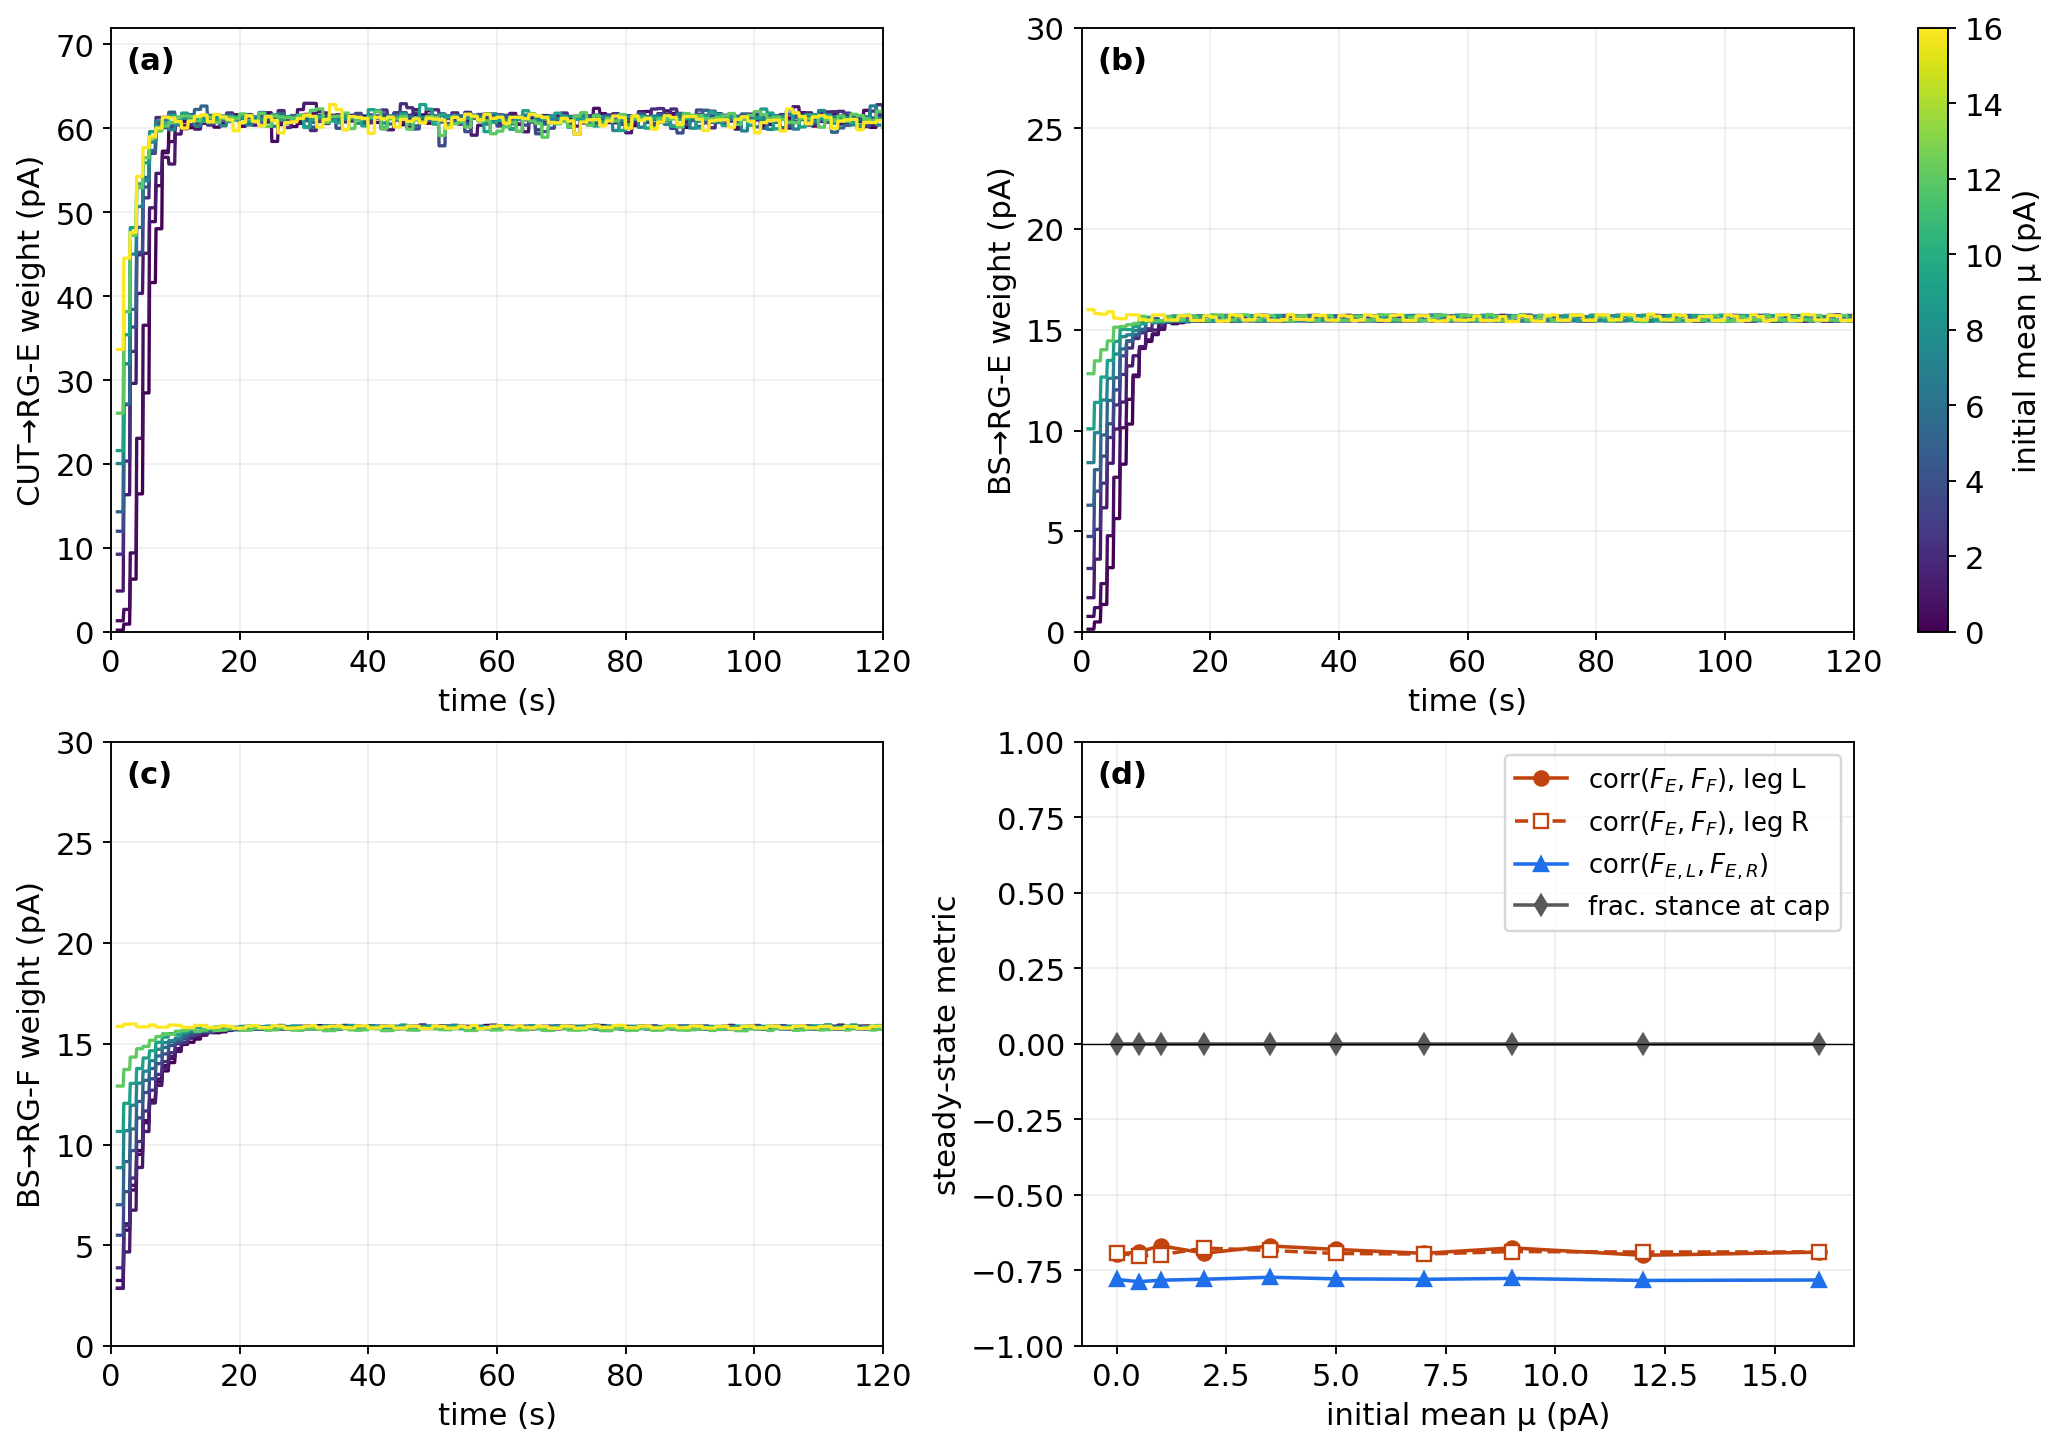
\includegraphics[width=\textwidth]{fig_init_robustness.png}
  \caption{\textbf{Initialisation robustness of force-triggered stepping.}
    Medium walk, $\lambda=10^{-3}$, ten STDP initial-weight distributions
    ($\mu=0$--$16$\,pA; colour). \textbf{(a--c)} Weight trajectories of
    CUT$\to$RG-E, BS$\to$RG-E and BS$\to$RG-F (leg L, pA) versus time (s).
    \textbf{(d)} Steady-state ($t\ge30$\,s) gait metrics versus initial mean
    weight: extensor/flexor force correlation per leg, left/right extensor
    force correlation, and the fraction of stance bouts ended by the timeout.}
  \label{fig:init_robustness}
\end{figure}

\subsection{The learned synapses settle at values that do not depend on the walking mode}\label{sec:results:weights}

We next vary the locomotion mode and the learning rate together, on a grid of
four modes by five rates. The modes are slow, medium and fast walk (full
weight-bearing; medium walk is also called \emph{plantar stepping} or
\emph{baseline}) and \emph{toe stepping} (partial body-weight support, sensory
feedback halved). Their operating points (Table~\ref{tab:modes}) give strides of
$1016\pm36$, $812\pm33$ and $594\pm24$\,ms for slow, medium and fast walk and
$845\pm66$\,ms for toe stepping at $\lambda=10^{-3}$ (last 20\,s). The
differences come from stance ($417$, $312$, $188$ and $360$\,ms), since swing
always lasts its timeout (\autoref{sec:methods:paced}). The learning rate
$\lambda$ sets how much each plastic synapse changes per correlated pre/post
spike pair and is swept across five decades,
$\lambda\in\{10^{-2},10^{-3},10^{-4},10^{-5},10^{-6}\}$.

Once learning has converged, the synapses reach the same values in every mode
(Figure~\ref{fig:weights_grid}; both legs in Supplementary
Figure~\ref{fig:weight_matrix}): CUT$\to$RG-E settles at $61$--$63$\,pA and
BS$\to$RG-E/F at $15$--$16$\,pA, and the left and right legs learn the same
values. The learning rate sets how fast the synapses get there. At
$\lambda=10^{-3}$, CUT$\to$RG-E reaches $90\%$ of its final value within
$\approx6$\,s in the three walking modes; at $10^{-4}$ it takes $50$--$64$\,s. At
the fastest rate ($10^{-2}$) the synapses jump to their range within a few
seconds but then fluctuate from step to step below the plateau
(CUT$\to$RG-E $\approx46$--$58$\,pA). At $10^{-5}$ and $10^{-6}$ they barely
move within the $120$\,s run (CUT$\to$RG-E reaching $\approx7$--$14$\,pA and
staying at its $\approx4$\,pA initial value, respectively). Partial unloading
slows learning, because the paw-contact drive that trains CUT$\to$RG-E is itself
weaker: toe stepping needs $14$\,s instead of $6$\,s at $\lambda=10^{-3}$, and at
$10^{-4}$ it has reached only $\approx47$--$50$\,pA by the end of the run.

\begin{figure}[t]
  \centering
  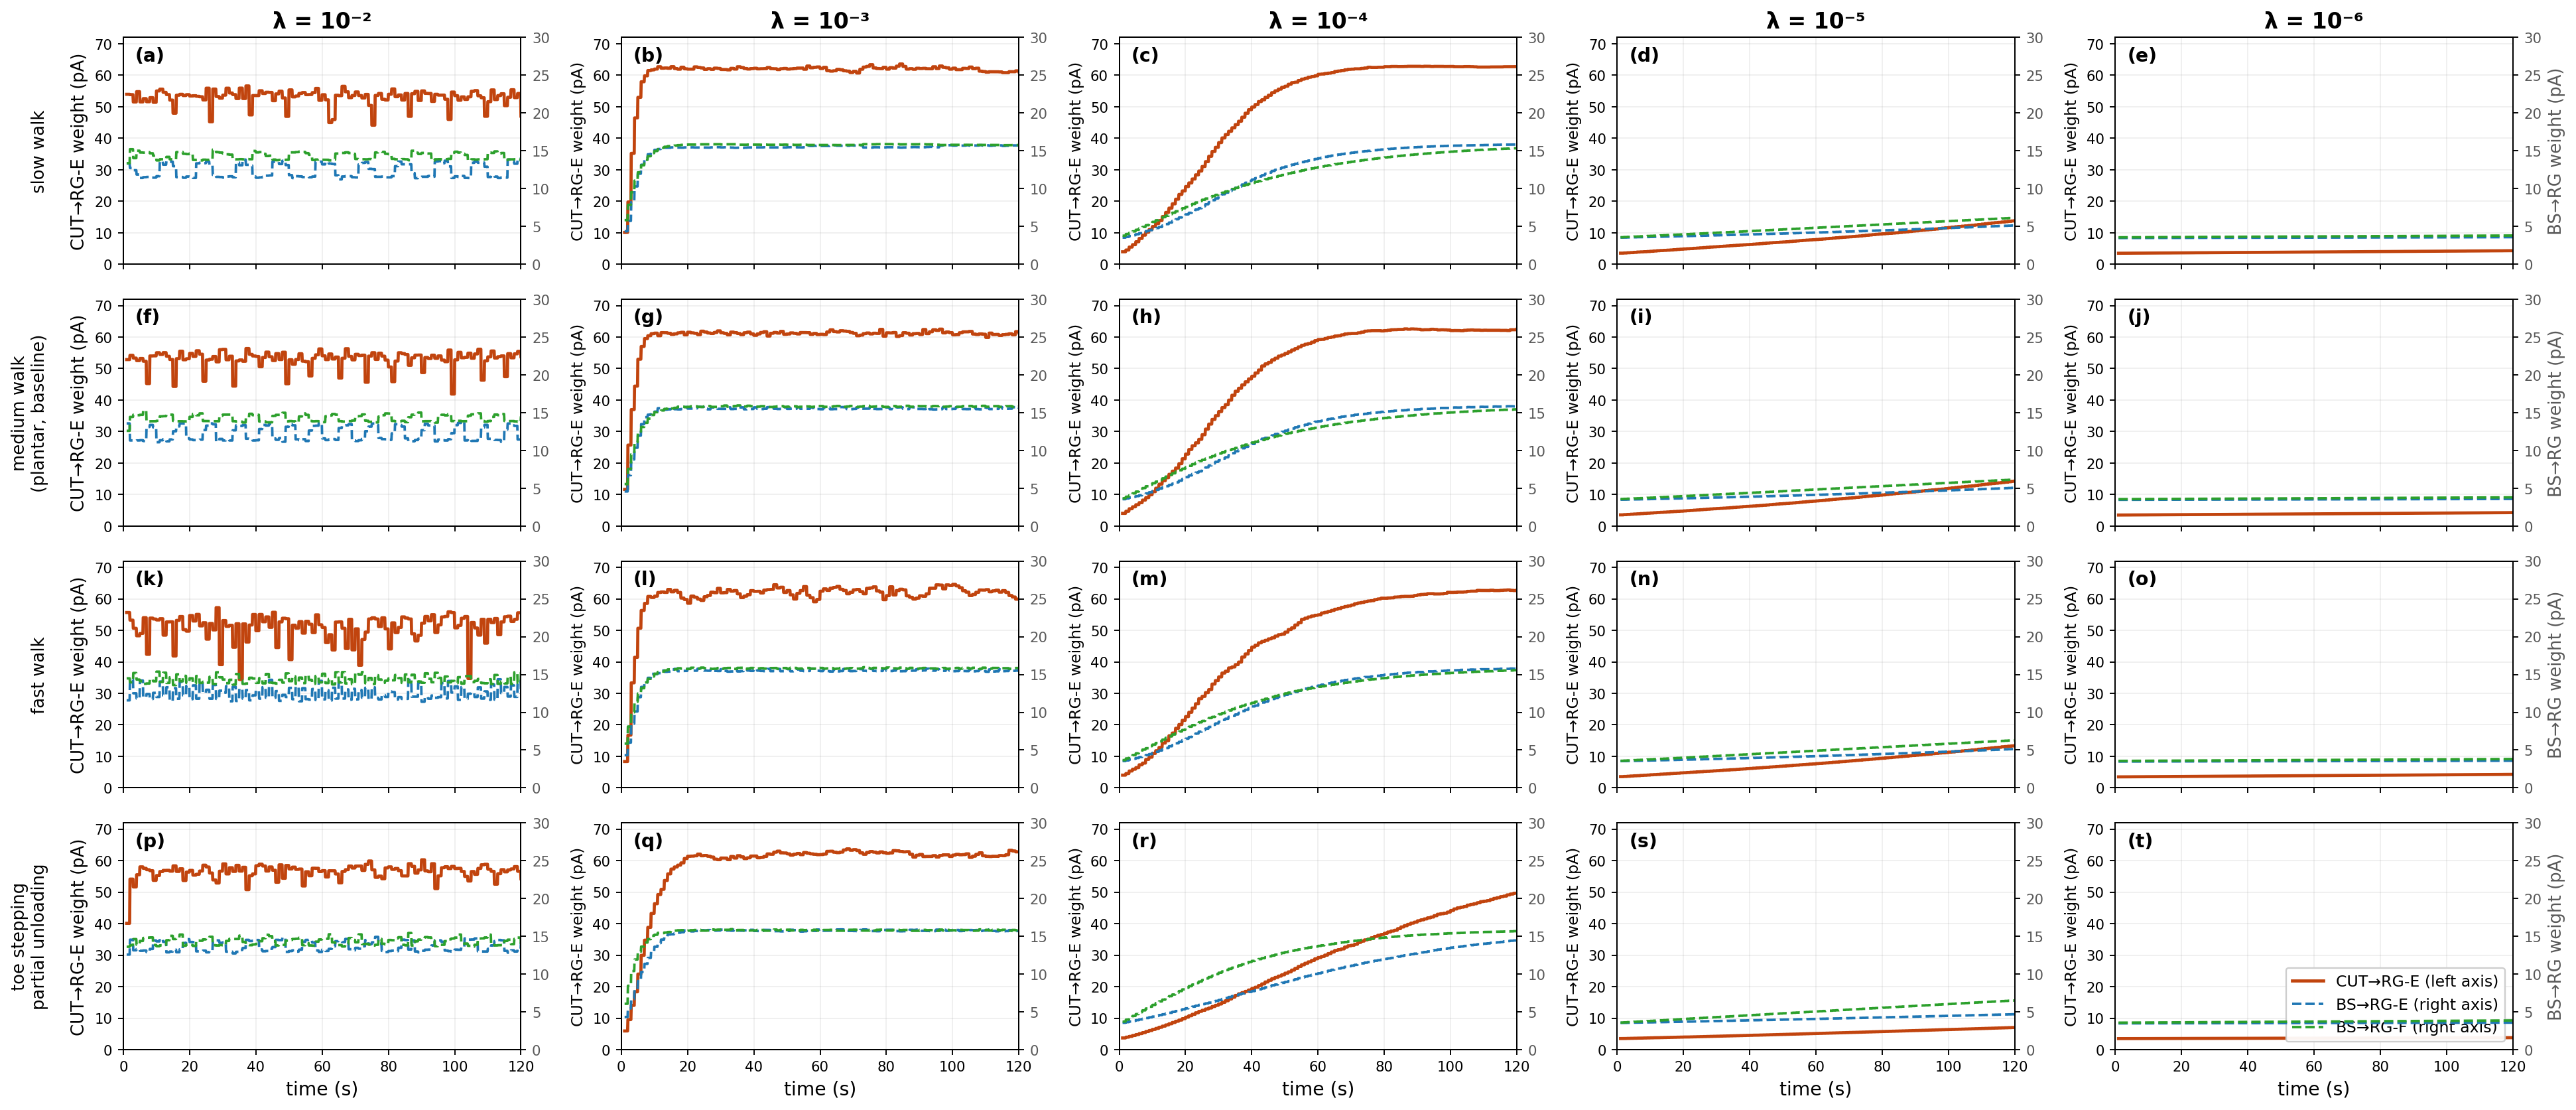
\includegraphics[width=0.95\textwidth]{fig_stdp_weights_grid.png}
  \caption{\textbf{Weight trajectories of the three plastic projections, per
    locomotion mode and learning rate.} Rows: the four locomotion modes;
    columns: the five learning rates. Each panel shows CUT$\to$RG-E (solid,
    left axis, pA) and BS$\to$RG-E, BS$\to$RG-F (dashed, right axis, pA) for leg
    L versus time (s). Panels (a)--(t). The learning rate sets the time to
    plateau; partial unloading (bottom row) slows CUT$\to$RG-E convergence.}
  \label{fig:weights_grid}
\end{figure}

% =============================================================
\subsection{Rehabilitation progress: the gait forms as the weights converge}\label{sec:results:force}

We next examine whether the learned wiring produces good walking, and how the
gait builds up over a session. Figures~\ref{fig:force_l2}--\ref{fig:force_l6}
show the extensor and flexor muscle forces in three short windows --- the
beginning, middle and end of each $120$\,s run --- one figure per learning rate,
so that reading a figure left-to-right traces how the gait develops as the
synapses strengthen. With learning that converges within the run
($\lambda=10^{-2}$ to $10^{-4}$) the forces settle into a regular alternation in
every mode, and stance ends on the force threshold (no stance bout at the
timeout over the last 20\,s). The alternation is clearest in slow and medium walk
(corr$(F_E,F_F)\approx-0.65$ to $-0.75$ over the last 20\,s), somewhat weaker
in toe stepping ($-0.55$ to $-0.71$), and weakest in fast walk ($-0.47$ to
$-0.57$), where the short stance leaves the extensor little time to rise and
fall. Under partial unloading the gait visibly sharpens as the weight grows
(toe stepping at $\lambda=10^{-3}$: $r=-0.31$ in the first window, $-0.65$ in
the last). Extensor force peaks at $\approx4$--$7$\,a.u.: stance now ends when
fatigue has pulled force below the threshold, before it saturates.

At the two slowest rates the gait does not form. At $\lambda=10^{-5}$ the loop
still switches on the force threshold, but with the cutaneous synapse still
weak the alternation degrades (corr$(F_E,F_F)$ $-0.18$ to $-0.49$ in the walking
modes), and in toe stepping stance already runs to the timeout. At
$\lambda=10^{-6}$ the synapses stay at their initial values and, in every mode,
most stance bouts run to the timeout ($41$--$95\%$). The alternation that remains
there can look regular --- corr$(F_E,F_F)$ reaches $-0.79$ in slow walk --- but
it is imposed by the timeouts acting as a clock, not produced by the sensory
loop.

\begin{figure}[t]
  \centering
  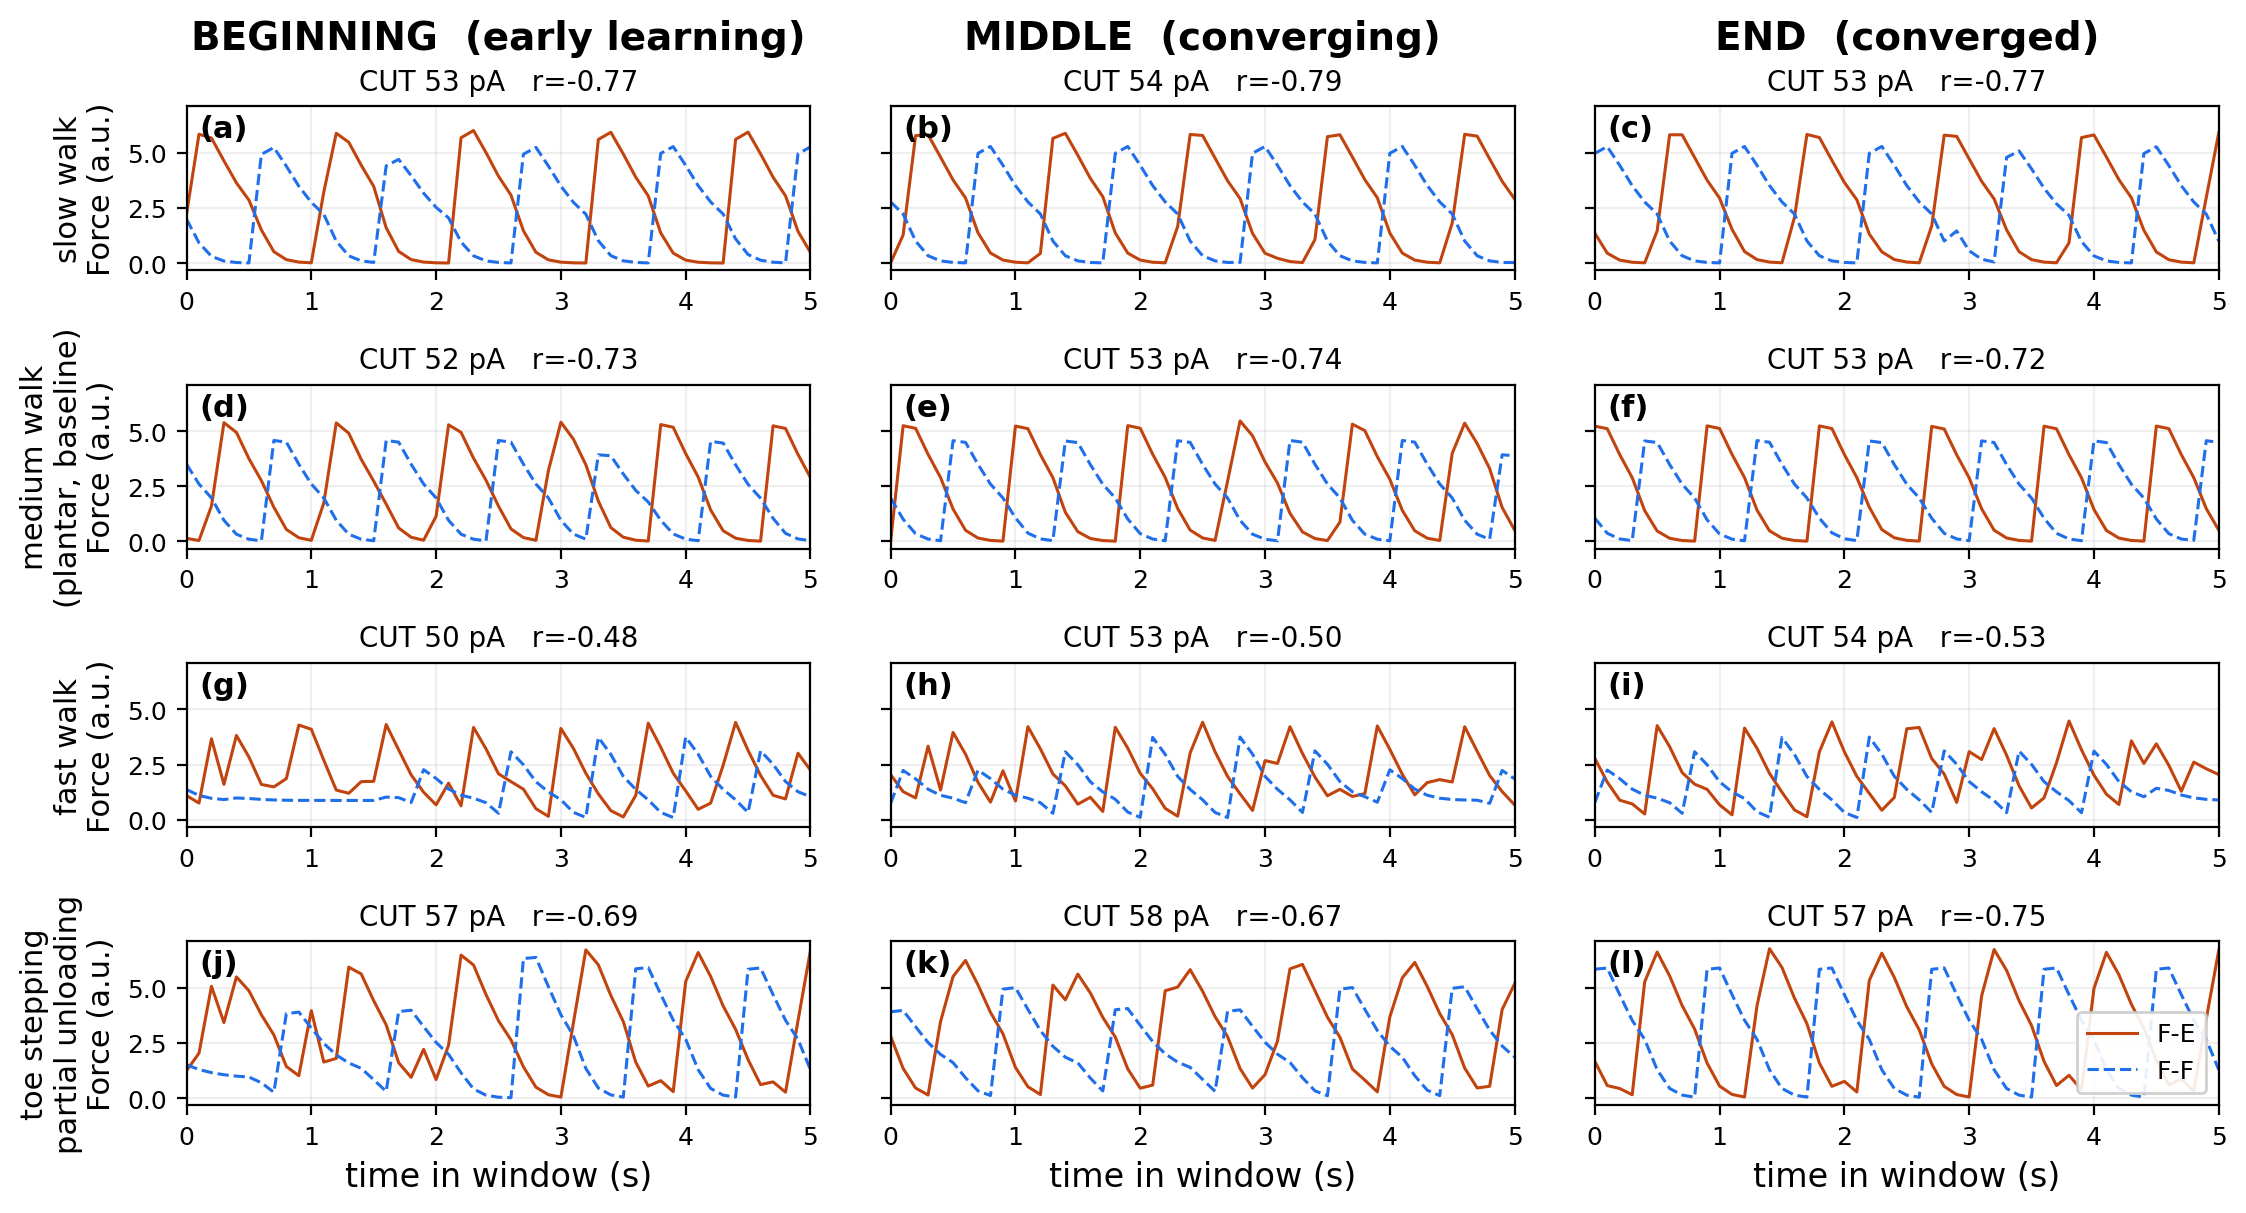
\includegraphics[width=0.9\textwidth]{fig_force_stages_lam1em2.png}
  \caption{\textbf{Force at three learning stages, four locomotion modes,
    $\lambda=10^{-2}$ (fastest rate).} Rows: the four locomotion modes; columns:
    beginning / middle / end of the $120$\,s run. Solid = Force-E, dashed =
    Force-F (a.u.)\ versus time (s), leg L; panels annotated with the mean
    CUT$\to$RG-E weight and in-window corr$(F_E,F_F)$. Panels (a)--(l).}
  \label{fig:force_l2}
\end{figure}

\begin{figure}[t]
  \centering
  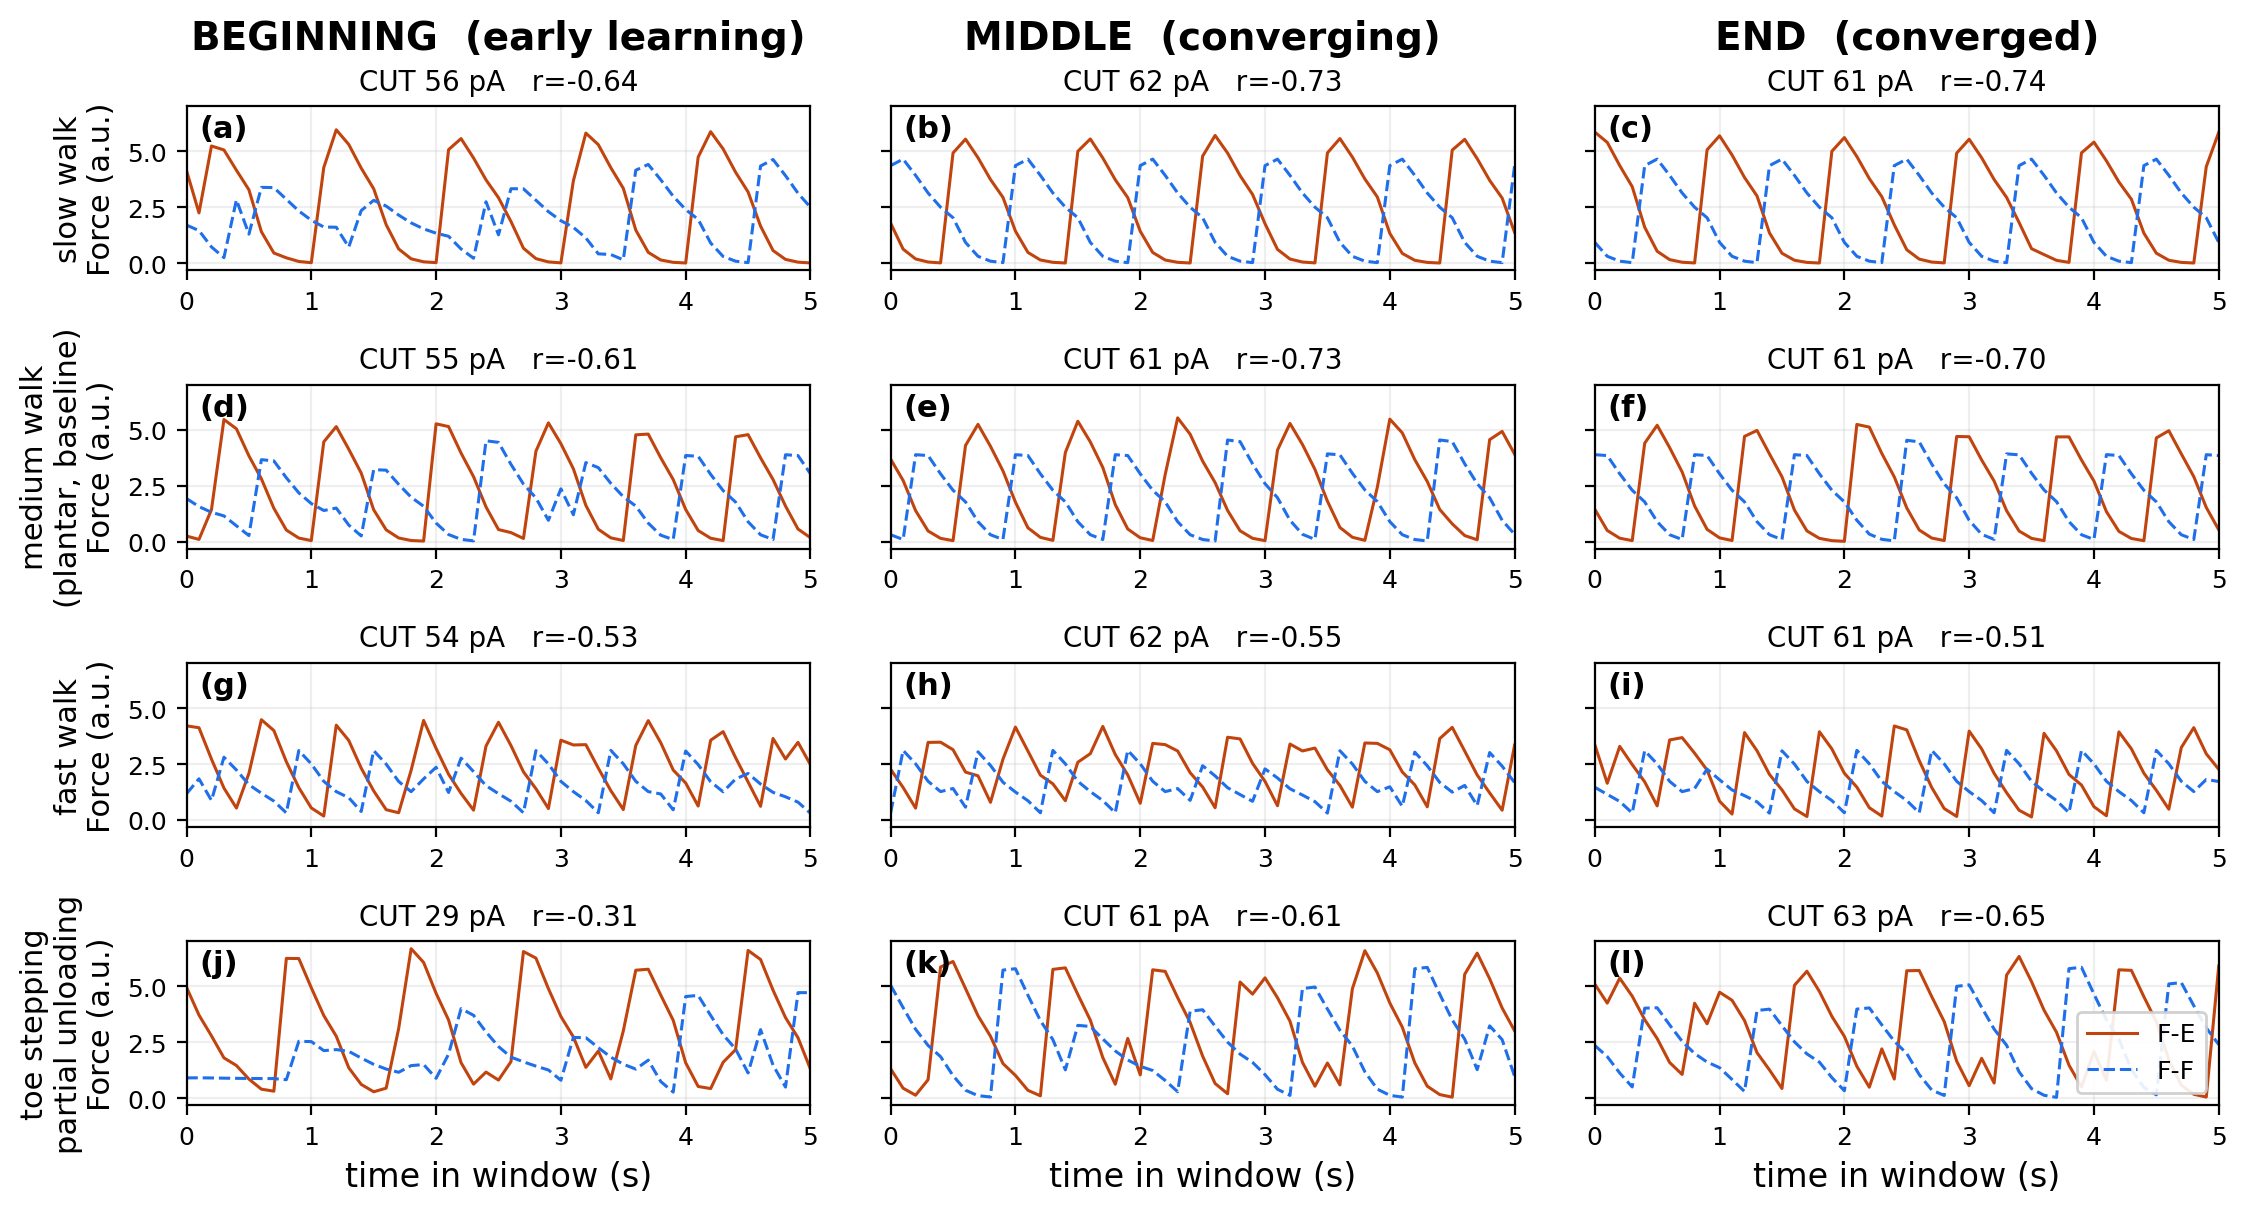
\includegraphics[width=0.9\textwidth]{fig_force_stages_lam1em3.png}
  \caption{\textbf{Force at three learning stages, four locomotion modes,
    $\lambda=10^{-3}$.} Same layout as Figure~\ref{fig:force_l2}.}
  \label{fig:force_l3}
\end{figure}

\begin{figure}[t]
  \centering
  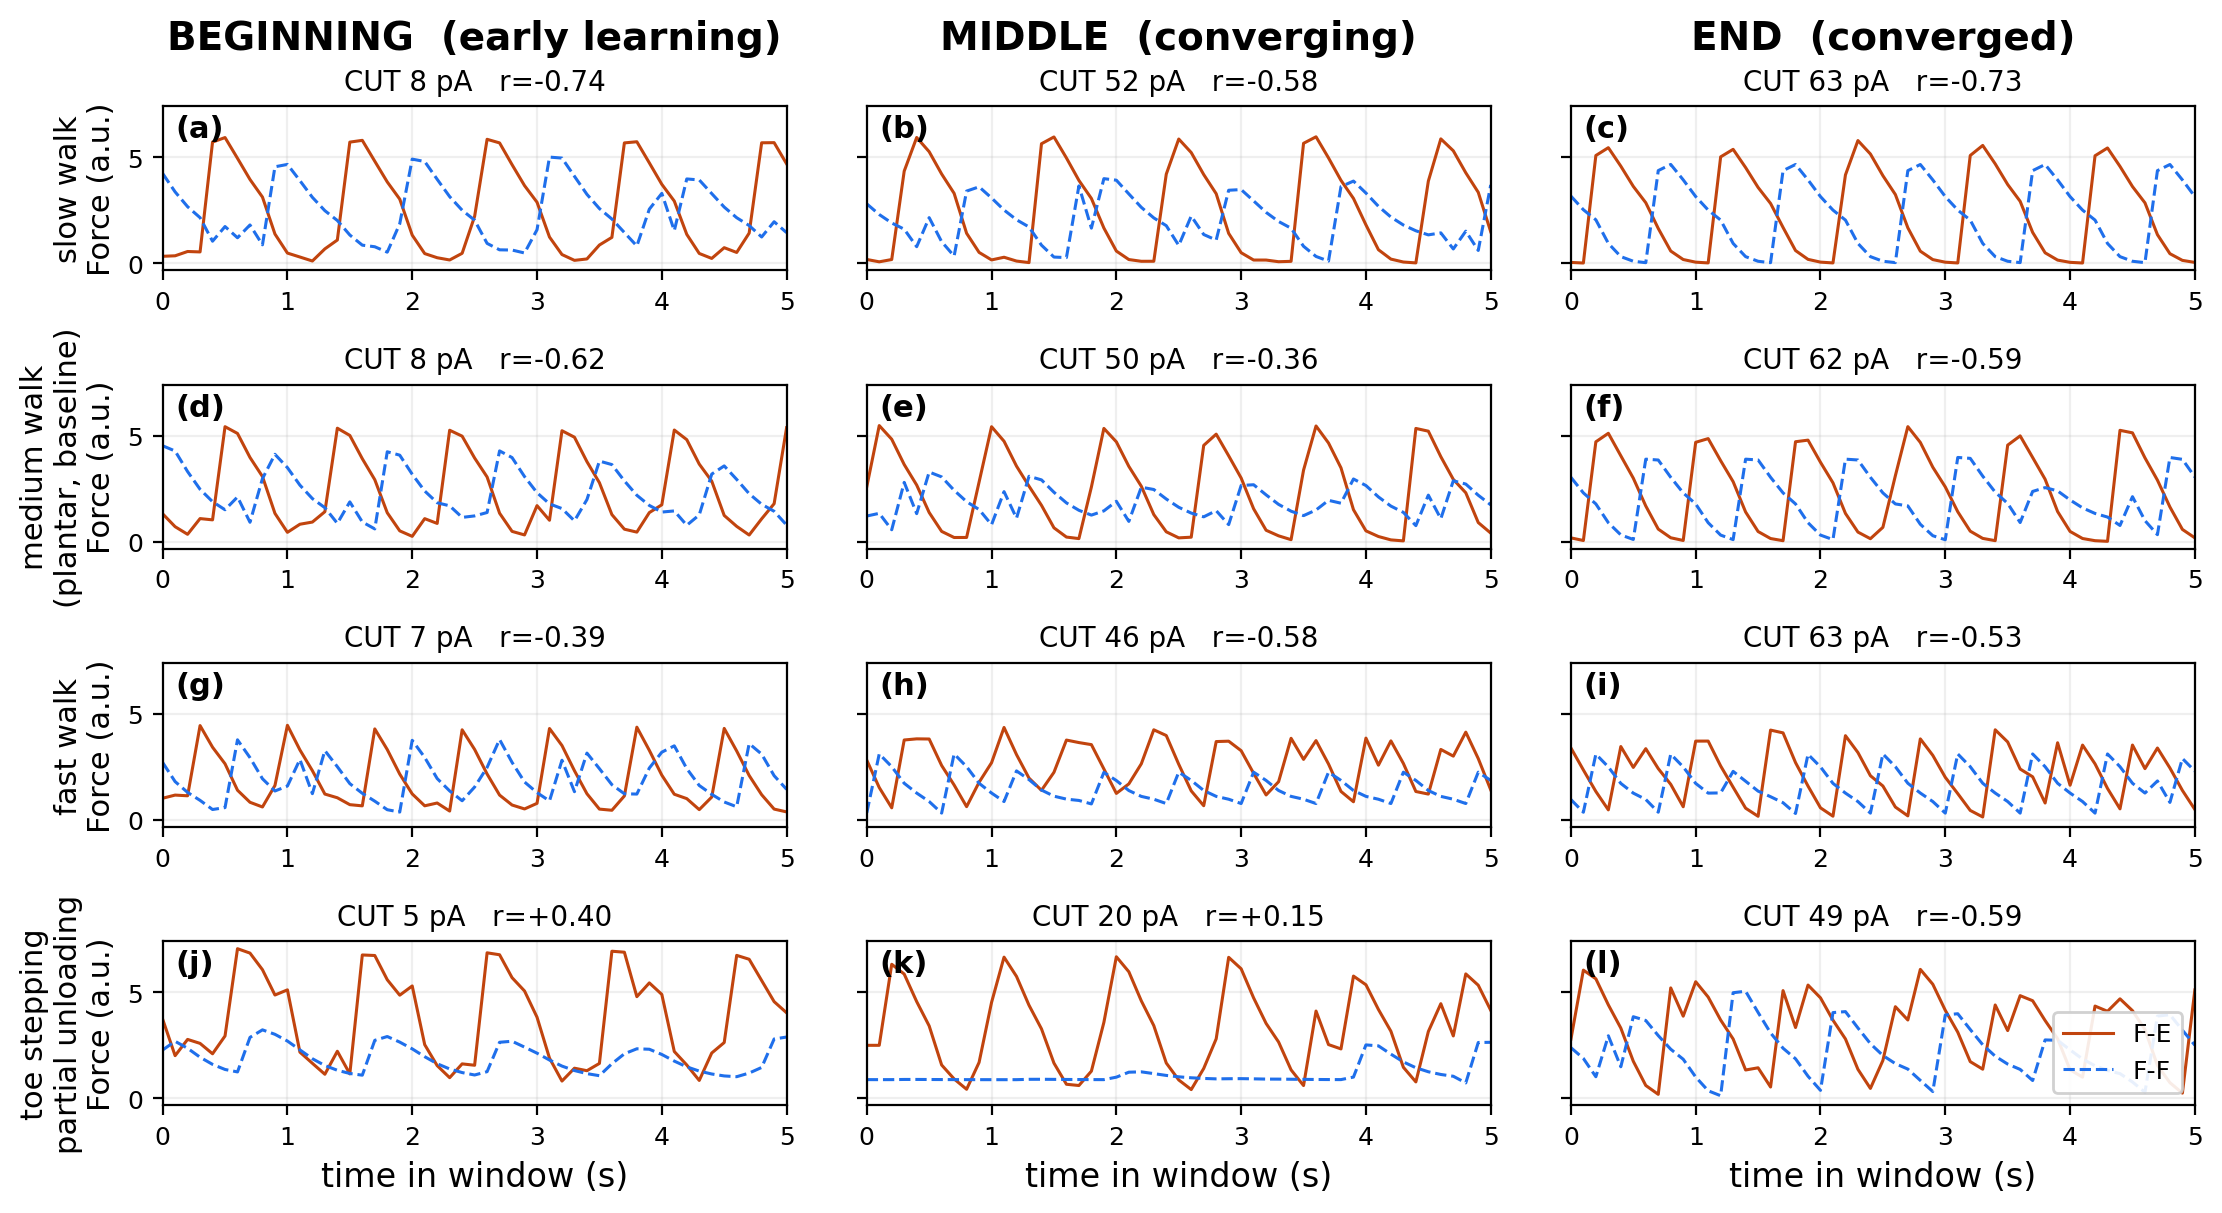
\includegraphics[width=0.9\textwidth]{fig_force_stages_lam1em4.png}
  \caption{\textbf{Force at three learning stages, four locomotion modes,
    $\lambda=10^{-4}$.} Same layout as Figure~\ref{fig:force_l2}. At this
    intermediate rate the three stages are most distinct, spanning the
    convergence of the weights.}
  \label{fig:force_l4}
\end{figure}

\begin{figure}[t]
  \centering
  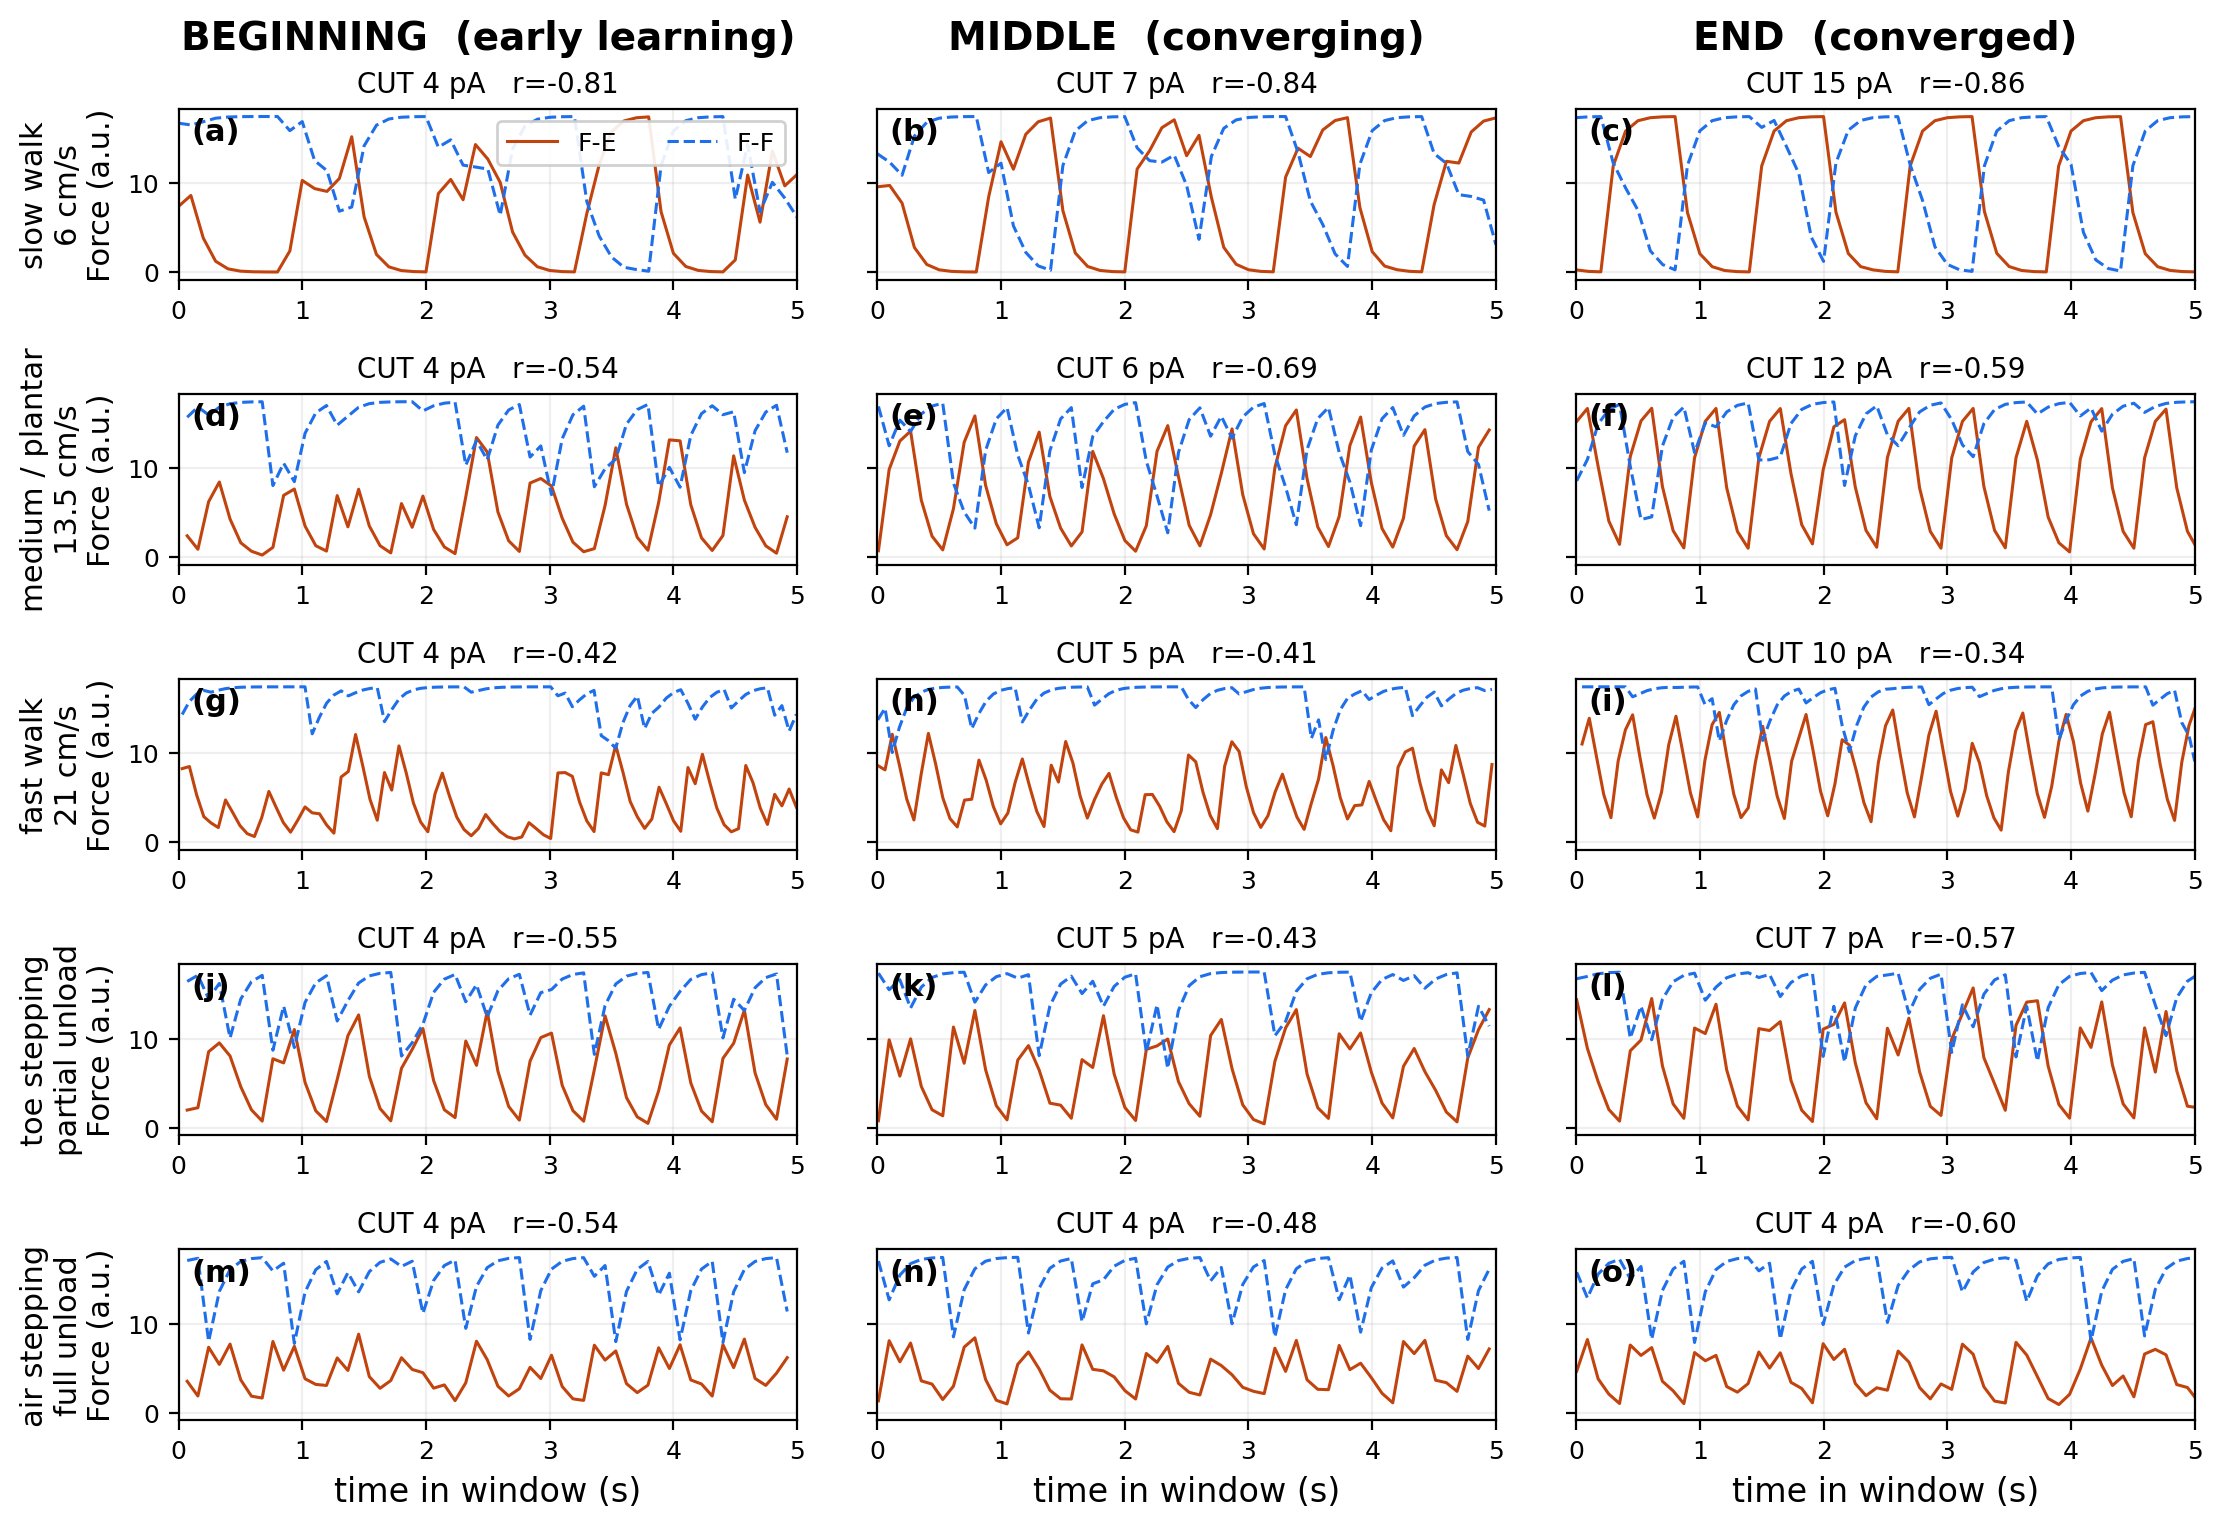
\includegraphics[width=0.9\textwidth]{fig_force_stages_lam1em5.png}
  \caption{\textbf{Force at three learning stages, four locomotion modes,
    $\lambda=10^{-5}$.} Same layout as Figure~\ref{fig:force_l2}. The
    cutaneous weight barely develops within the run and the alternation stays
    weak; in toe stepping stance runs to the timeout.}
  \label{fig:force_l5}
\end{figure}

\begin{figure}[t]
  \centering
  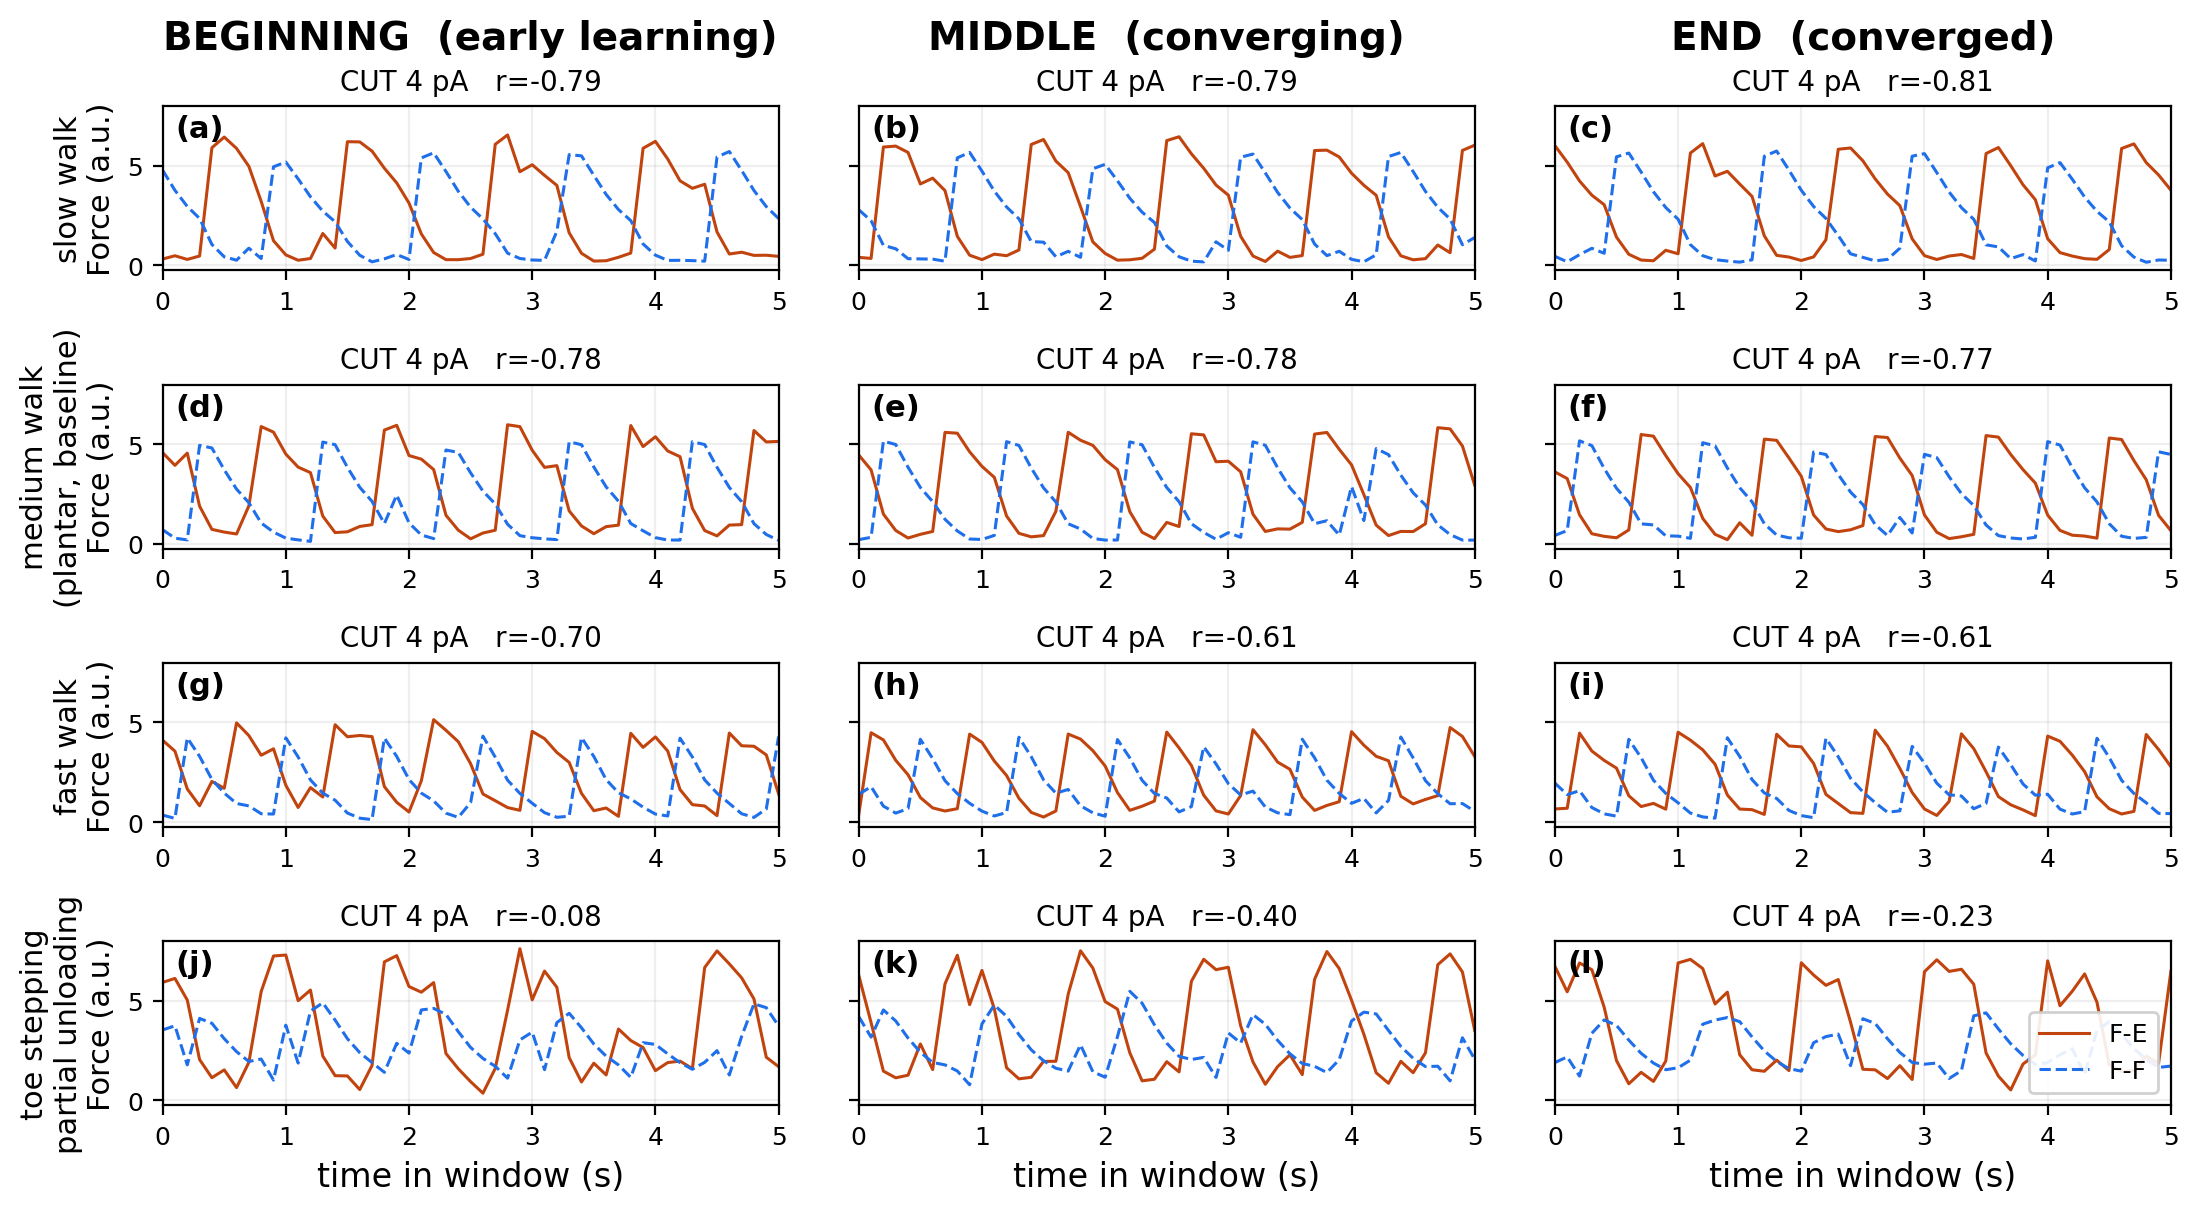
\includegraphics[width=0.9\textwidth]{fig_force_stages_lam1em6.png}
  \caption{\textbf{Force at three learning stages, four locomotion modes,
    $\lambda=10^{-6}$ (slowest rate).} Same layout as Figure~\ref{fig:force_l2}.
    The weights stay at their initial values; most stance bouts end at the
    timeout, so the regular pattern here is set by the timeouts rather than by
    the sensory loop.}
  \label{fig:force_l6}
\end{figure}

% =============================================================
\subsection{Network-level activity across the locomotion modes}\label{sec:results:network}

The muscle force is only the read-out of a whole network, so we next ask whether
the alternation is a property of the entire circuit.
Figures~\ref{fig:net_l2}--\ref{fig:net_l6} show the firing rates of all sixteen
recorded neuron pools --- for both legs, the rhythm generators (RG-E, RG-F), the
reciprocal-inhibition interneurons (InE, InF), the proprioceptive interneurons
(IaInt-E, IaInt-F) and the motor pools (M-E, M-F) --- over the last 4\,s of each
run, one figure per learning rate. At the converging rates every extensor-side
pool fires in alternation with its flexor-side partner in all four modes, the
two legs stay in antiphase, and the rhythm generators alternate strongly
(corr(RG-E,RG-F) between $-0.87$ and $-0.98$) --- so the alternation is built
into the core circuit, not imposed only at the muscle. The cycle shortens from
slow to fast walk while the pattern keeps its shape. Under toe stepping the
extensor-side pools (RG-E, InE, M-E) and the Ia interneurons fire at roughly
half the rate of full weight-bearing, the network-level signature of the halved
sensory feedback, while the flexor side is unchanged.

\begin{figure}[t]
  \centering
  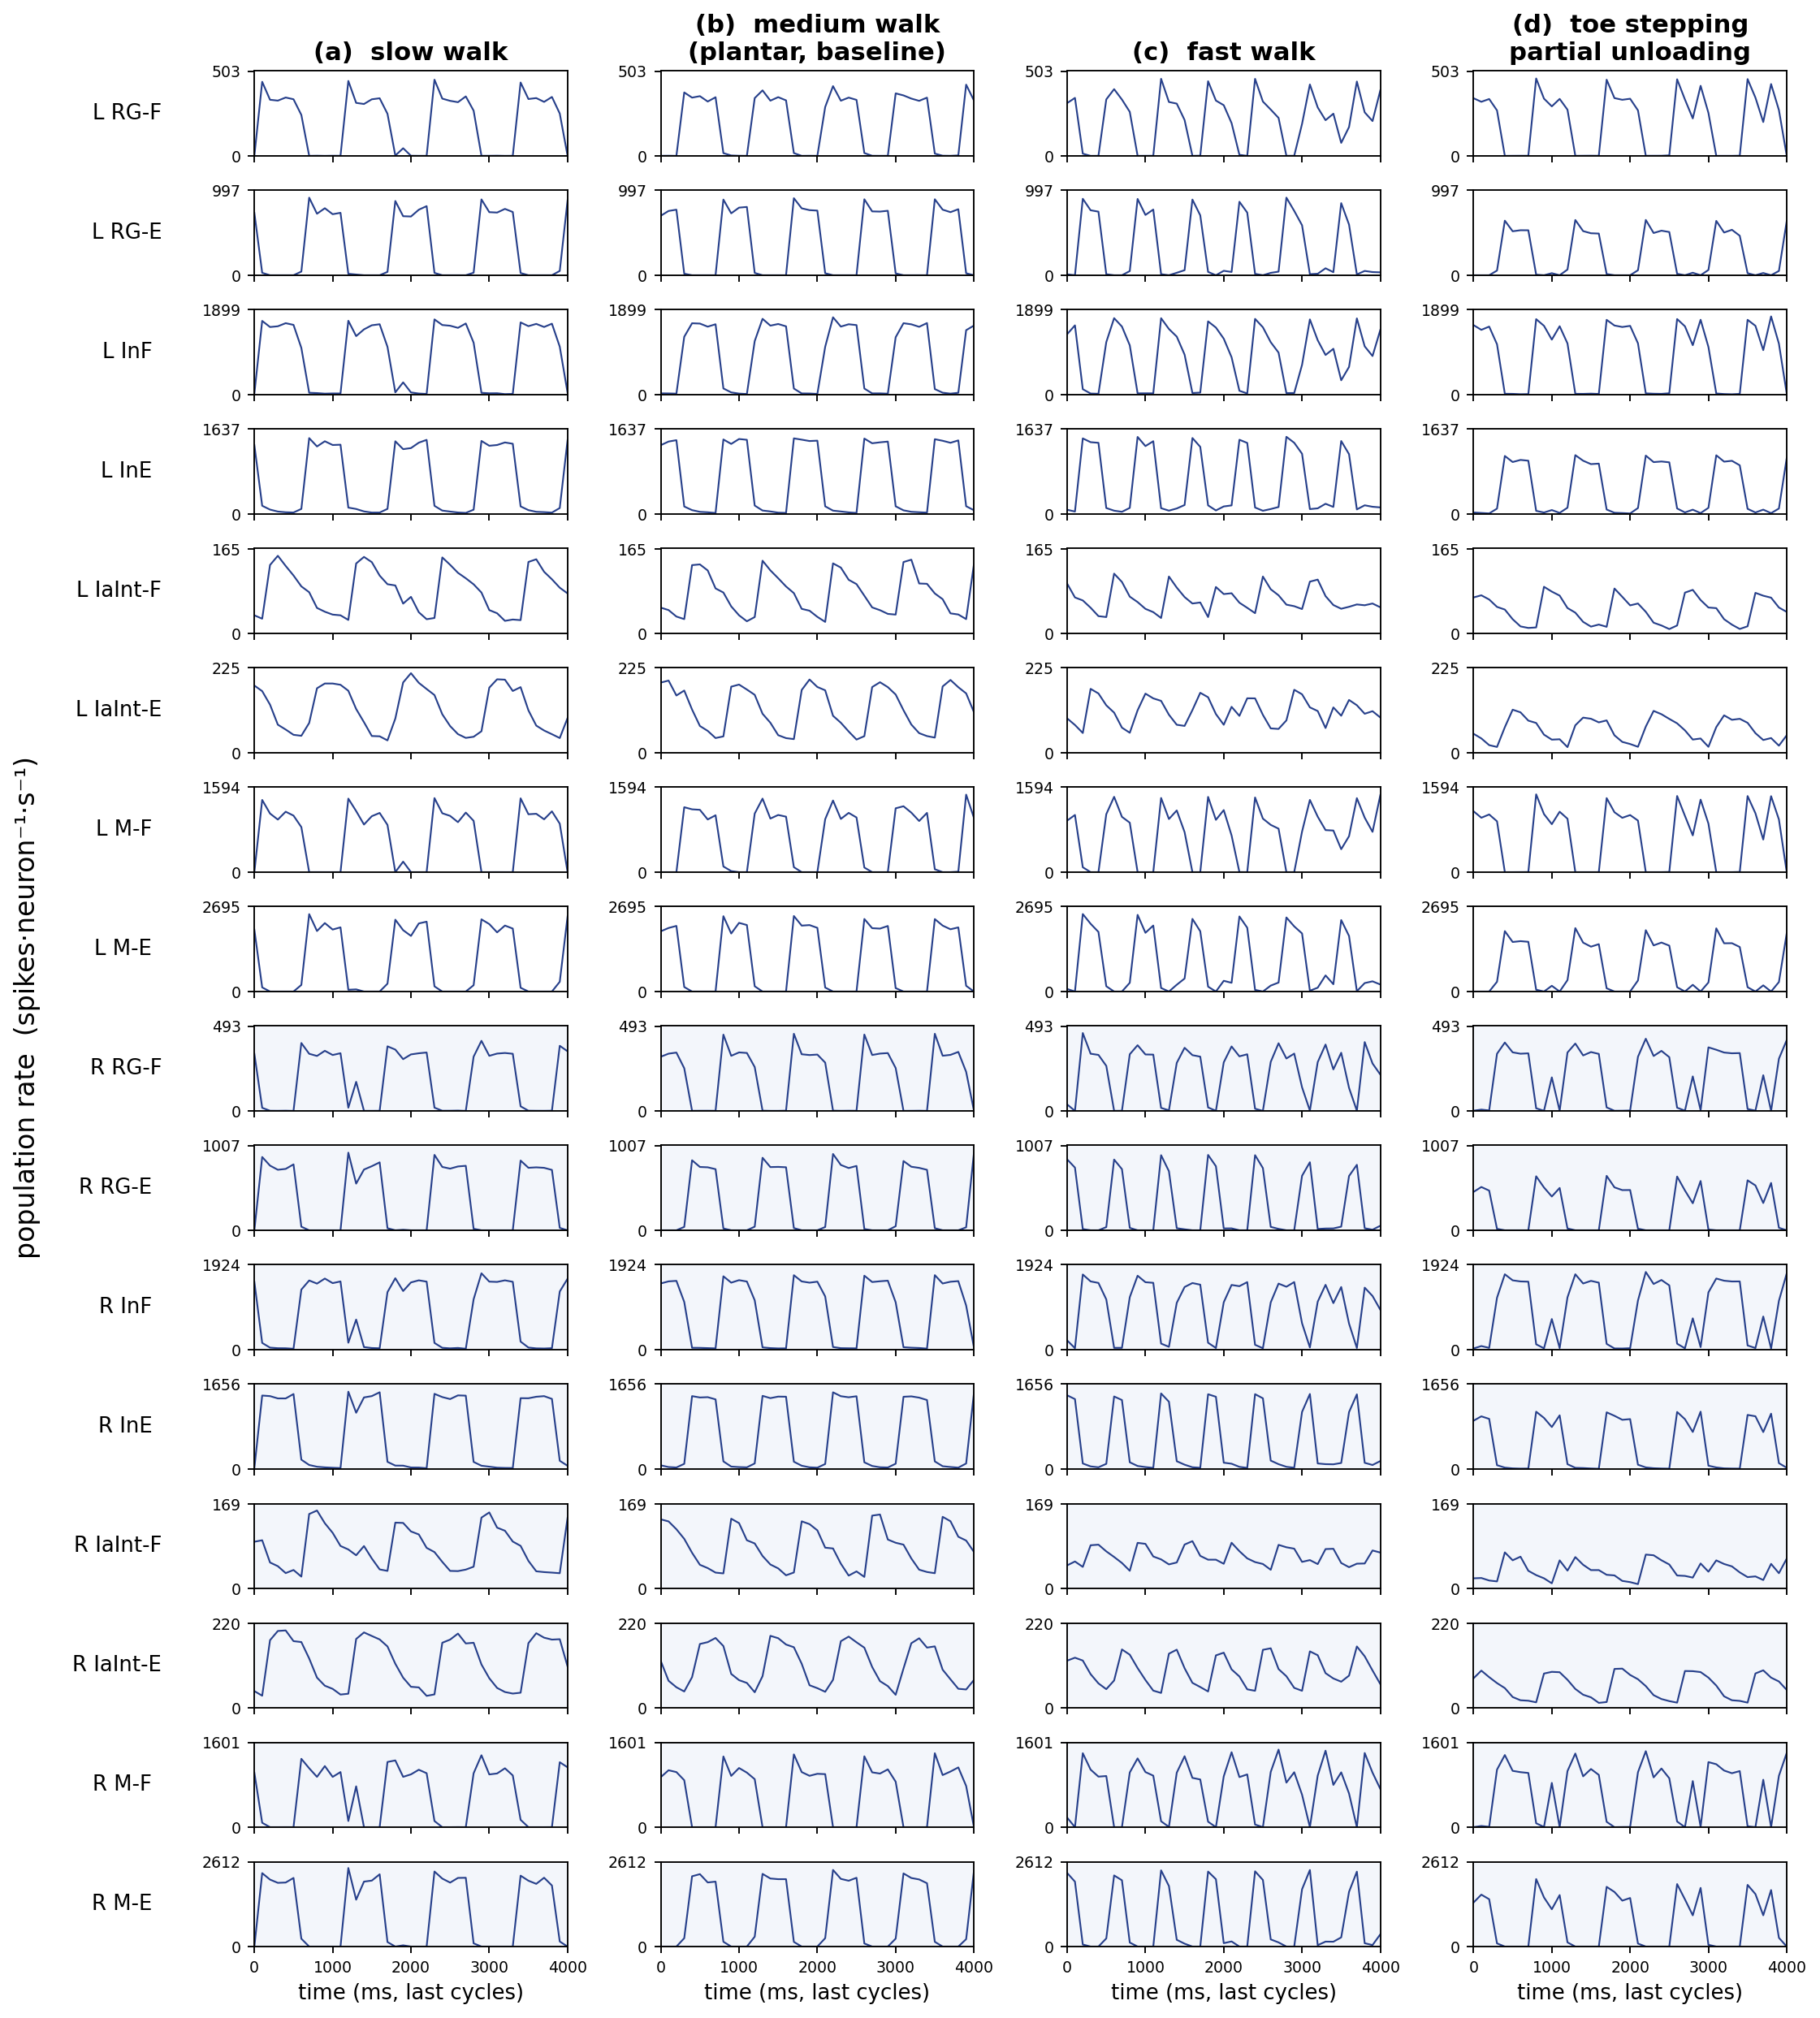
\includegraphics[width=0.95\textwidth]{fig_network_matrix_lam1em2.png}
  \caption{\textbf{Full-circuit population activity across the four locomotion
    modes, $\lambda=10^{-2}$ (fastest rate).} Rows: the sixteen recorded
    populations (both legs; right-leg rows tinted); columns (a)--(d): slow /
    medium (plantar, baseline) / fast walk and toe stepping. Population rate
    (spikes$\cdot$neuron$^{-1}\cdot$s$^{-1}$) versus time (ms), last 4\,s of
    the run.}
  \label{fig:net_l2}
\end{figure}

\begin{figure}[t]
  \centering
  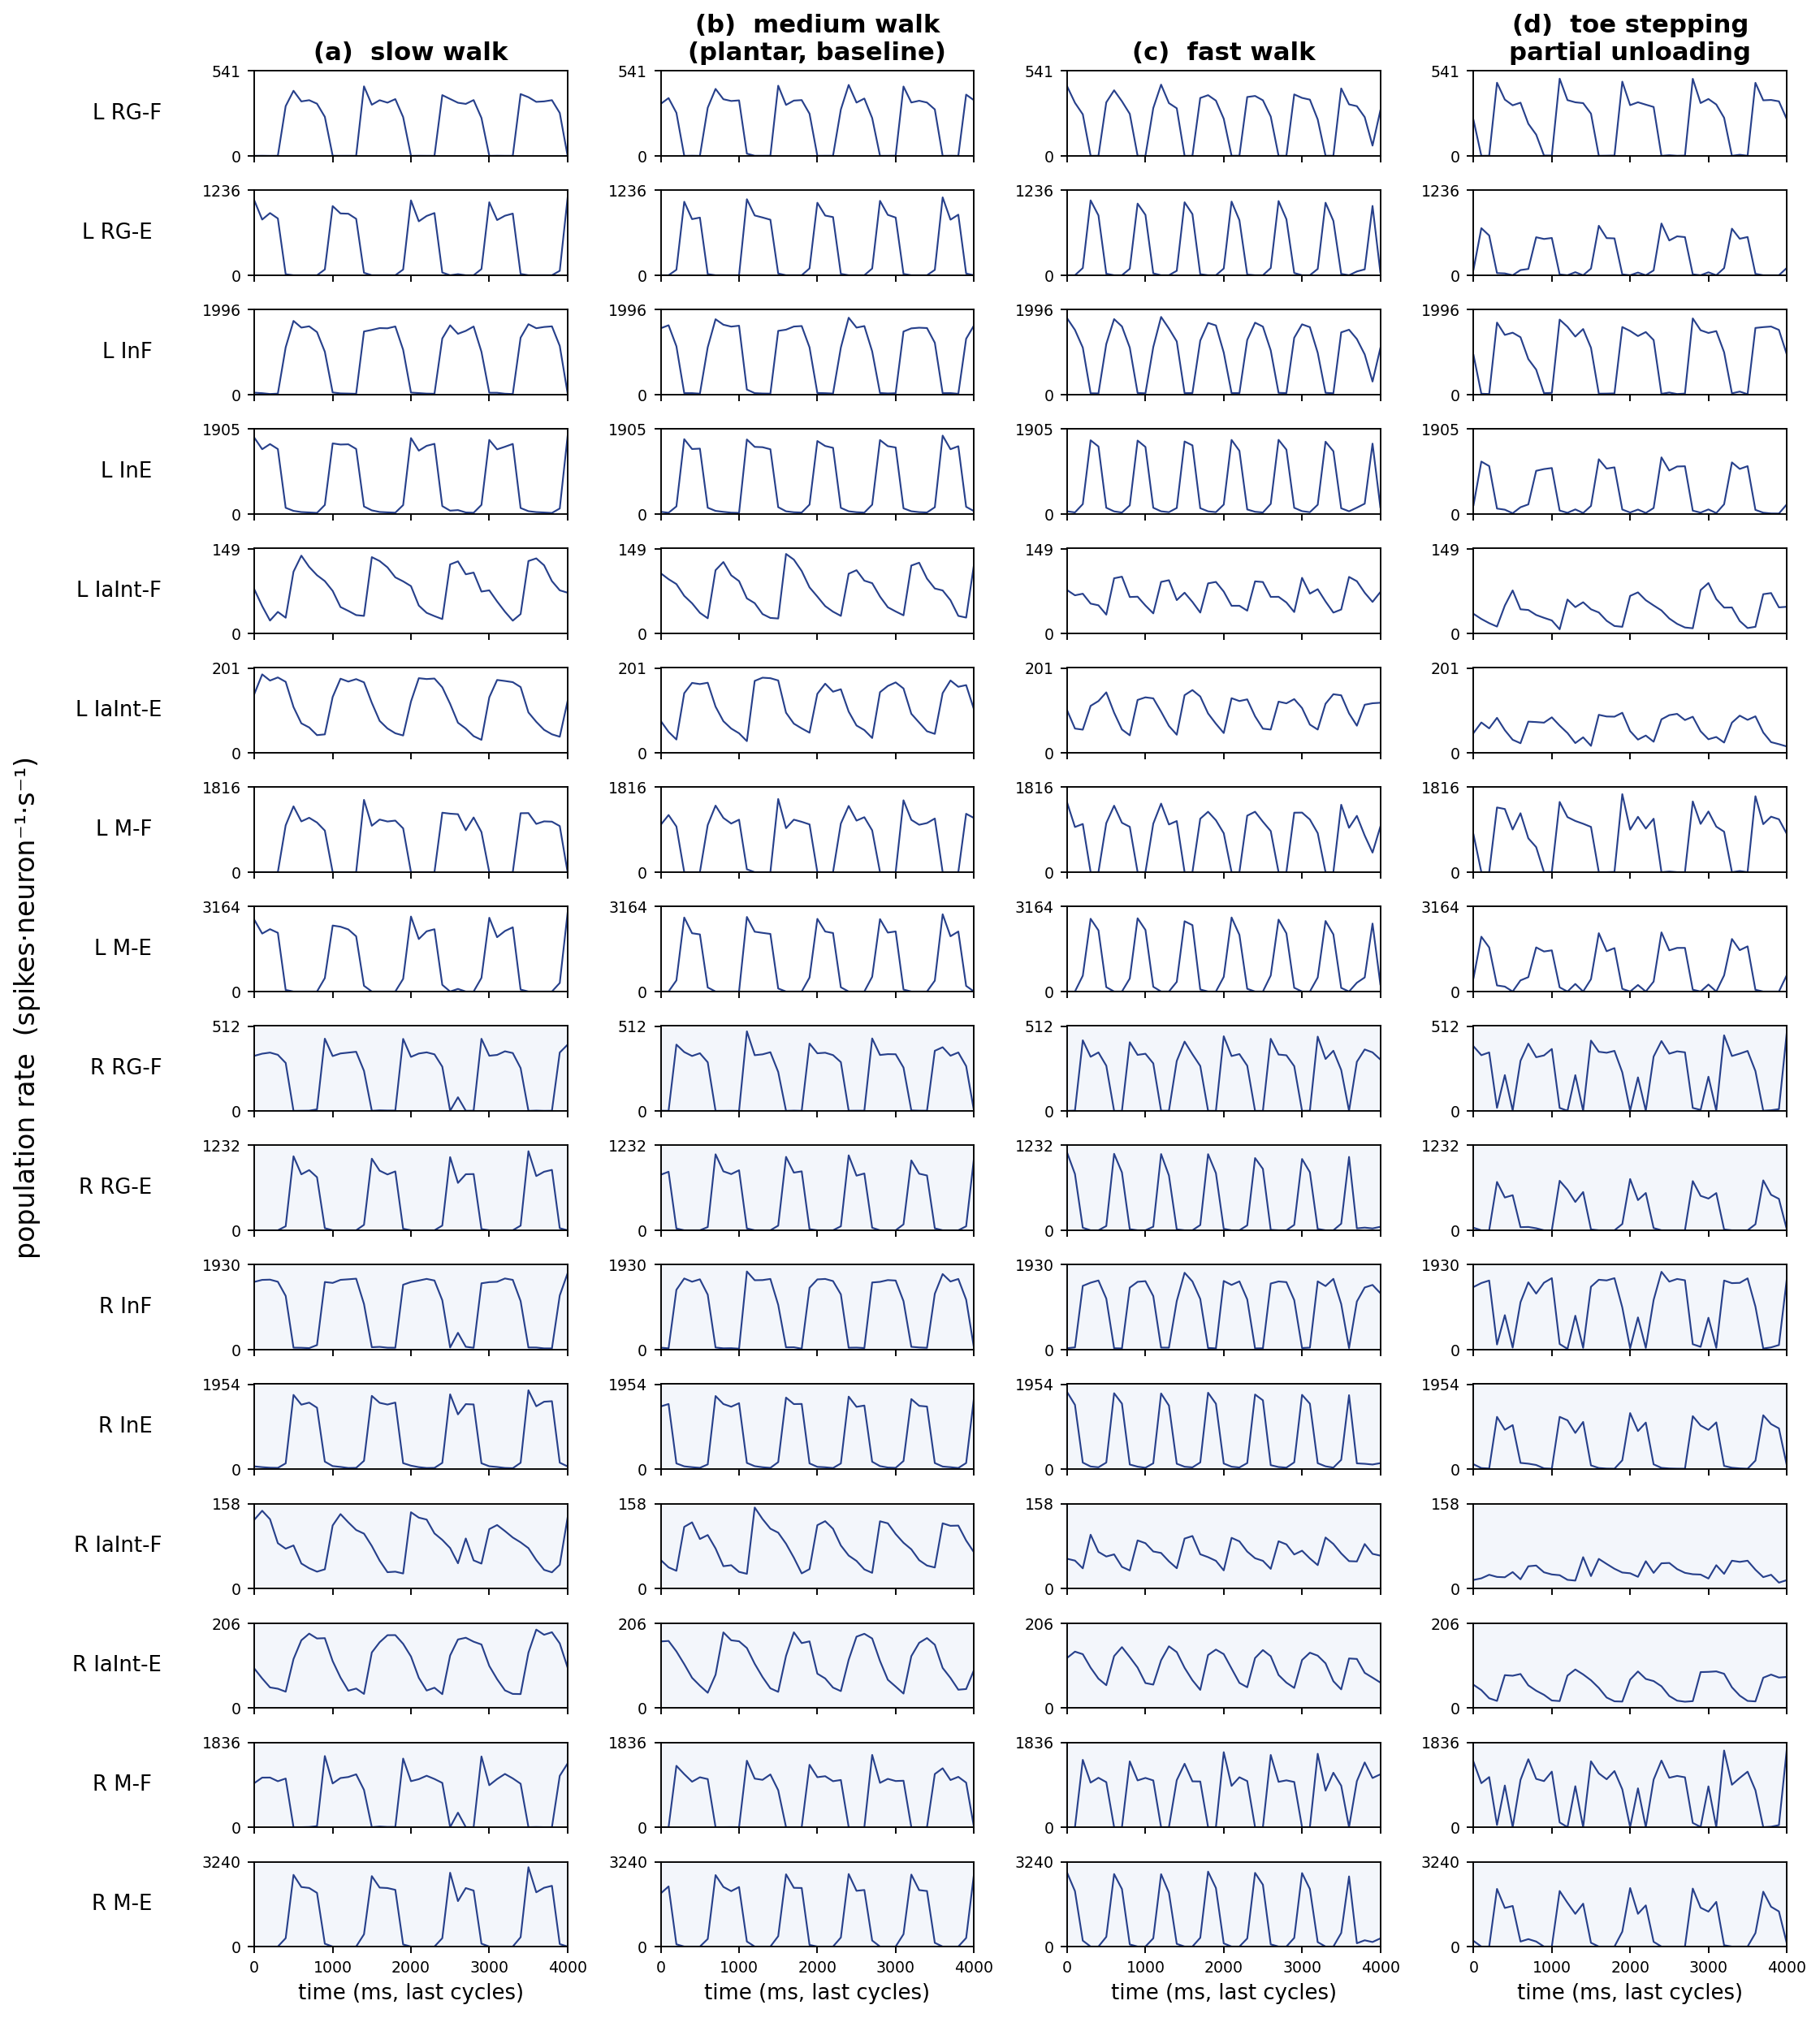
\includegraphics[width=0.95\textwidth]{fig_network_matrix_lam1em3.png}
  \caption{\textbf{Full-circuit population activity, $\lambda=10^{-3}$.} Same
    layout as Figure~\ref{fig:net_l2}.}
  \label{fig:net_l3}
\end{figure}

\begin{figure}[t]
  \centering
  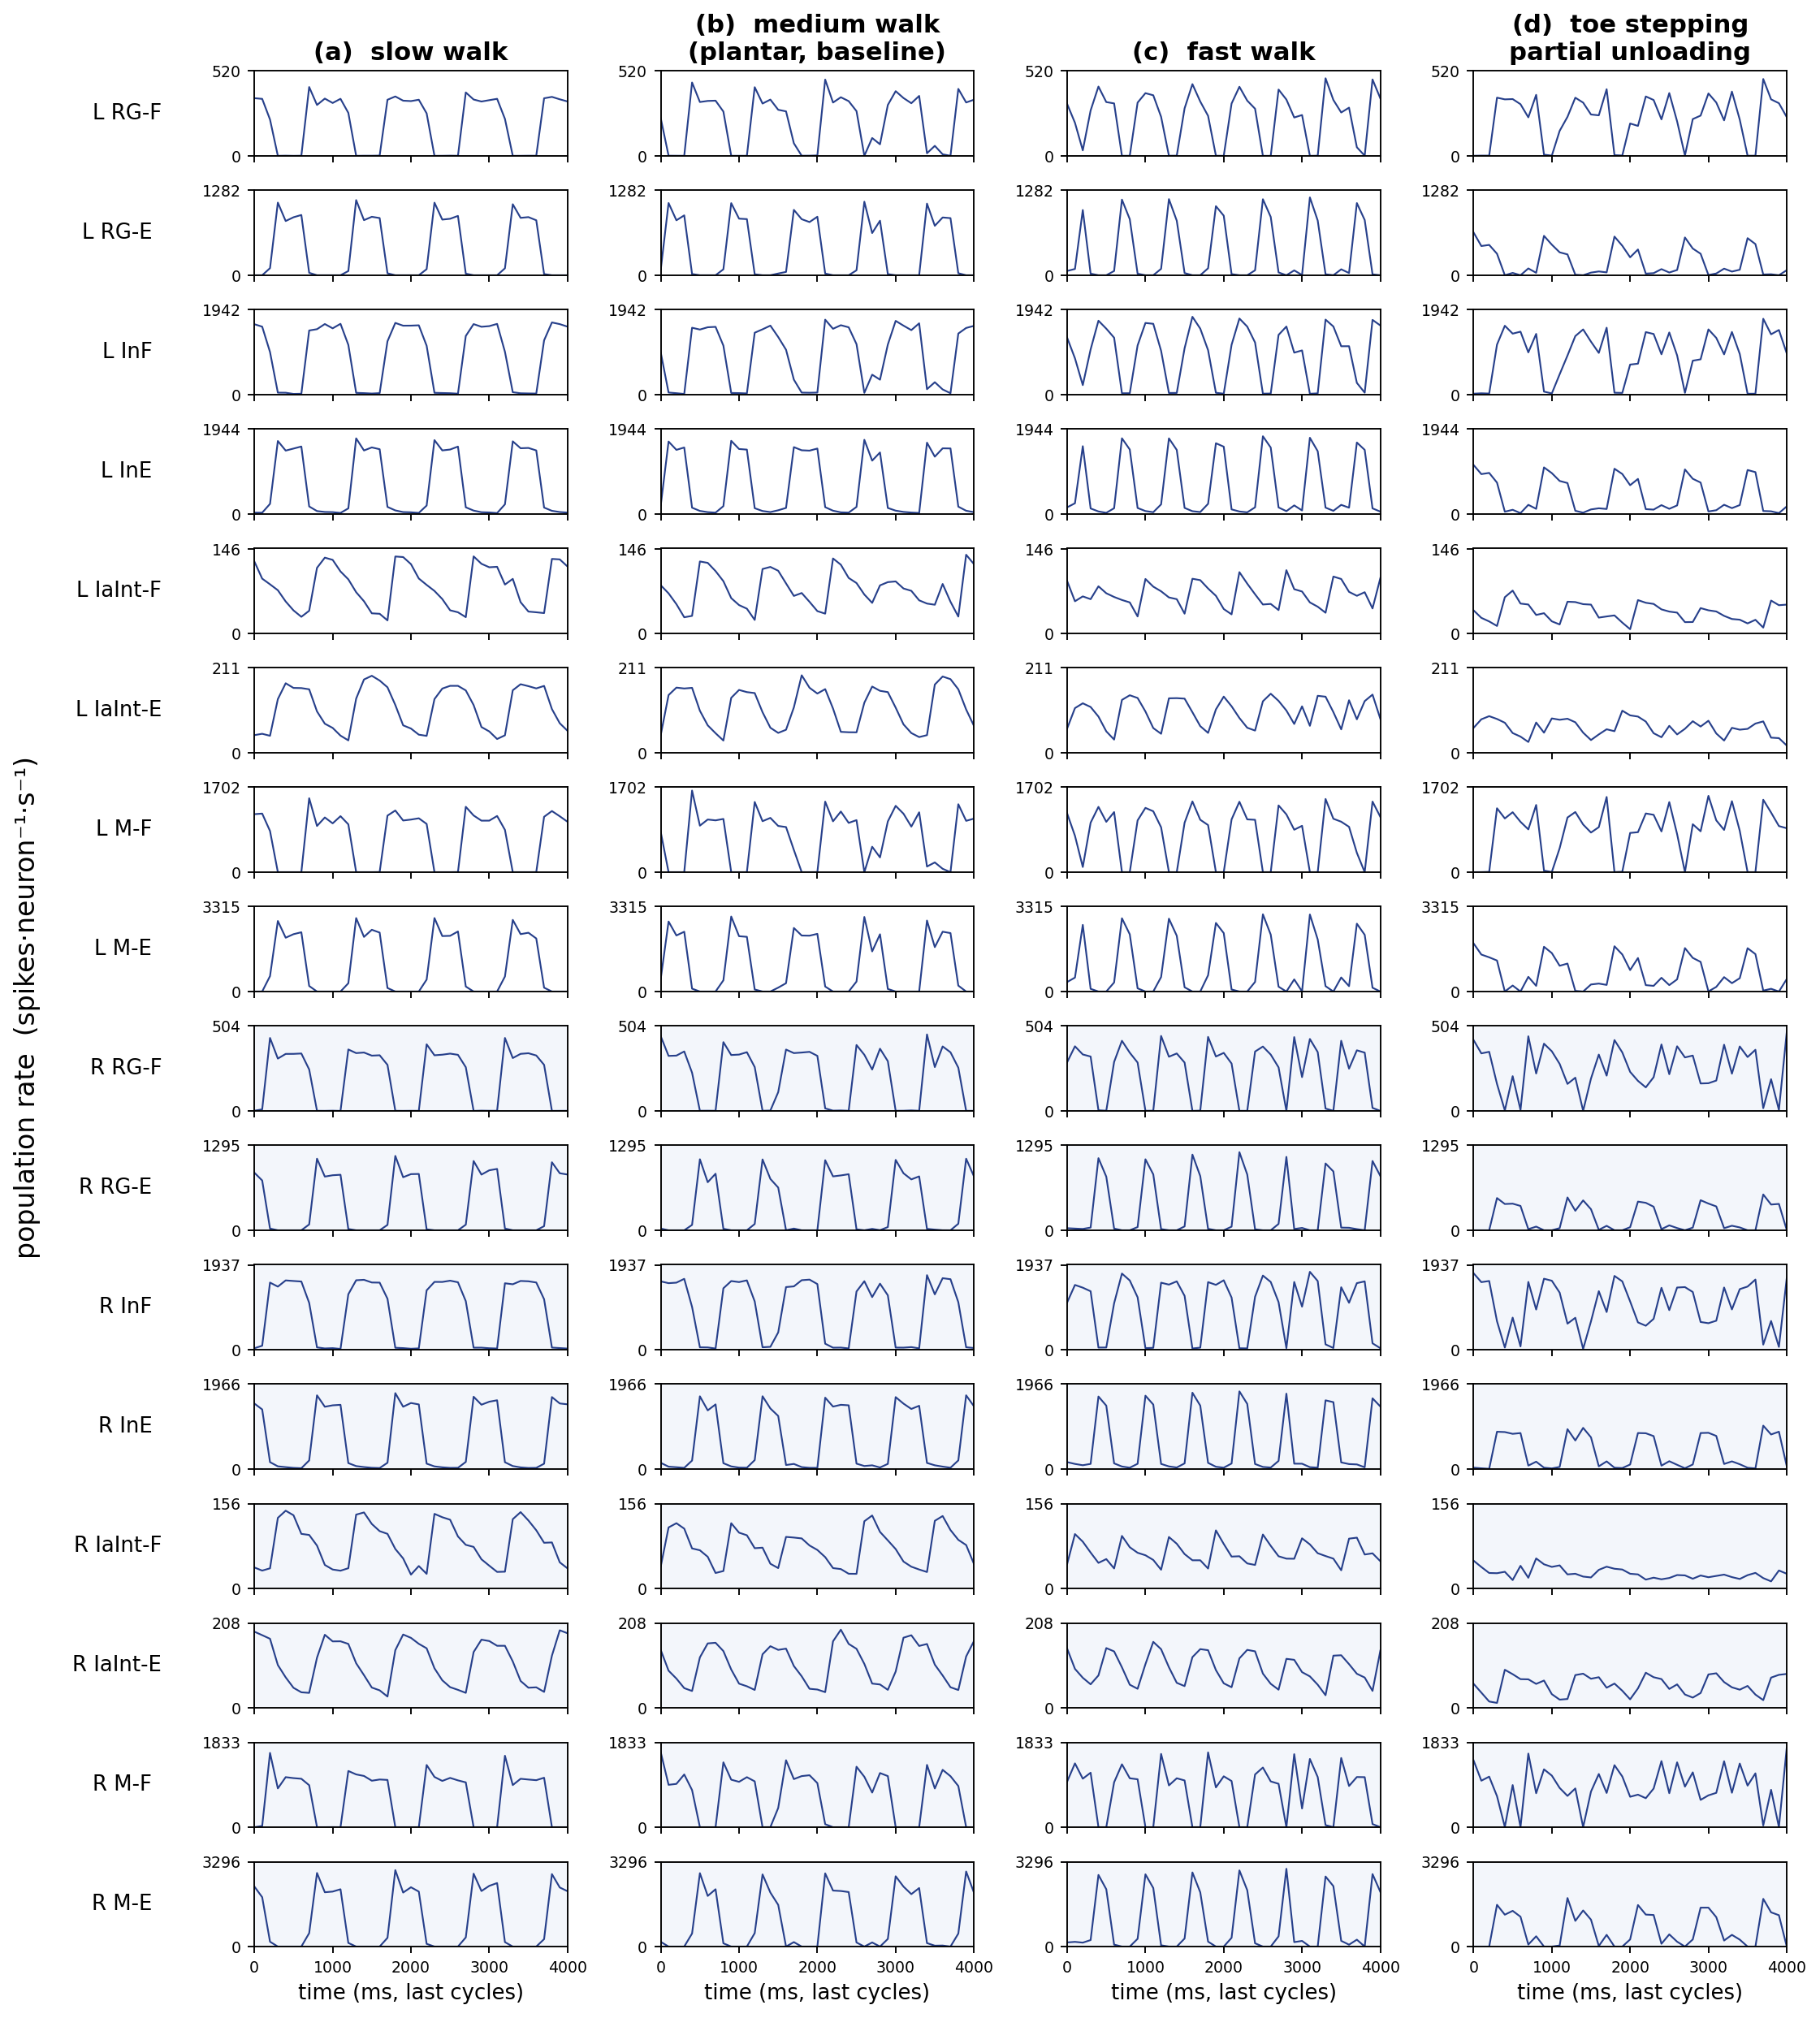
\includegraphics[width=0.95\textwidth]{fig_network_matrix_lam1em4.png}
  \caption{\textbf{Full-circuit population activity, $\lambda=10^{-4}$.} Same
    layout as Figure~\ref{fig:net_l2}.}
  \label{fig:net_l4}
\end{figure}

\begin{figure}[t]
  \centering
  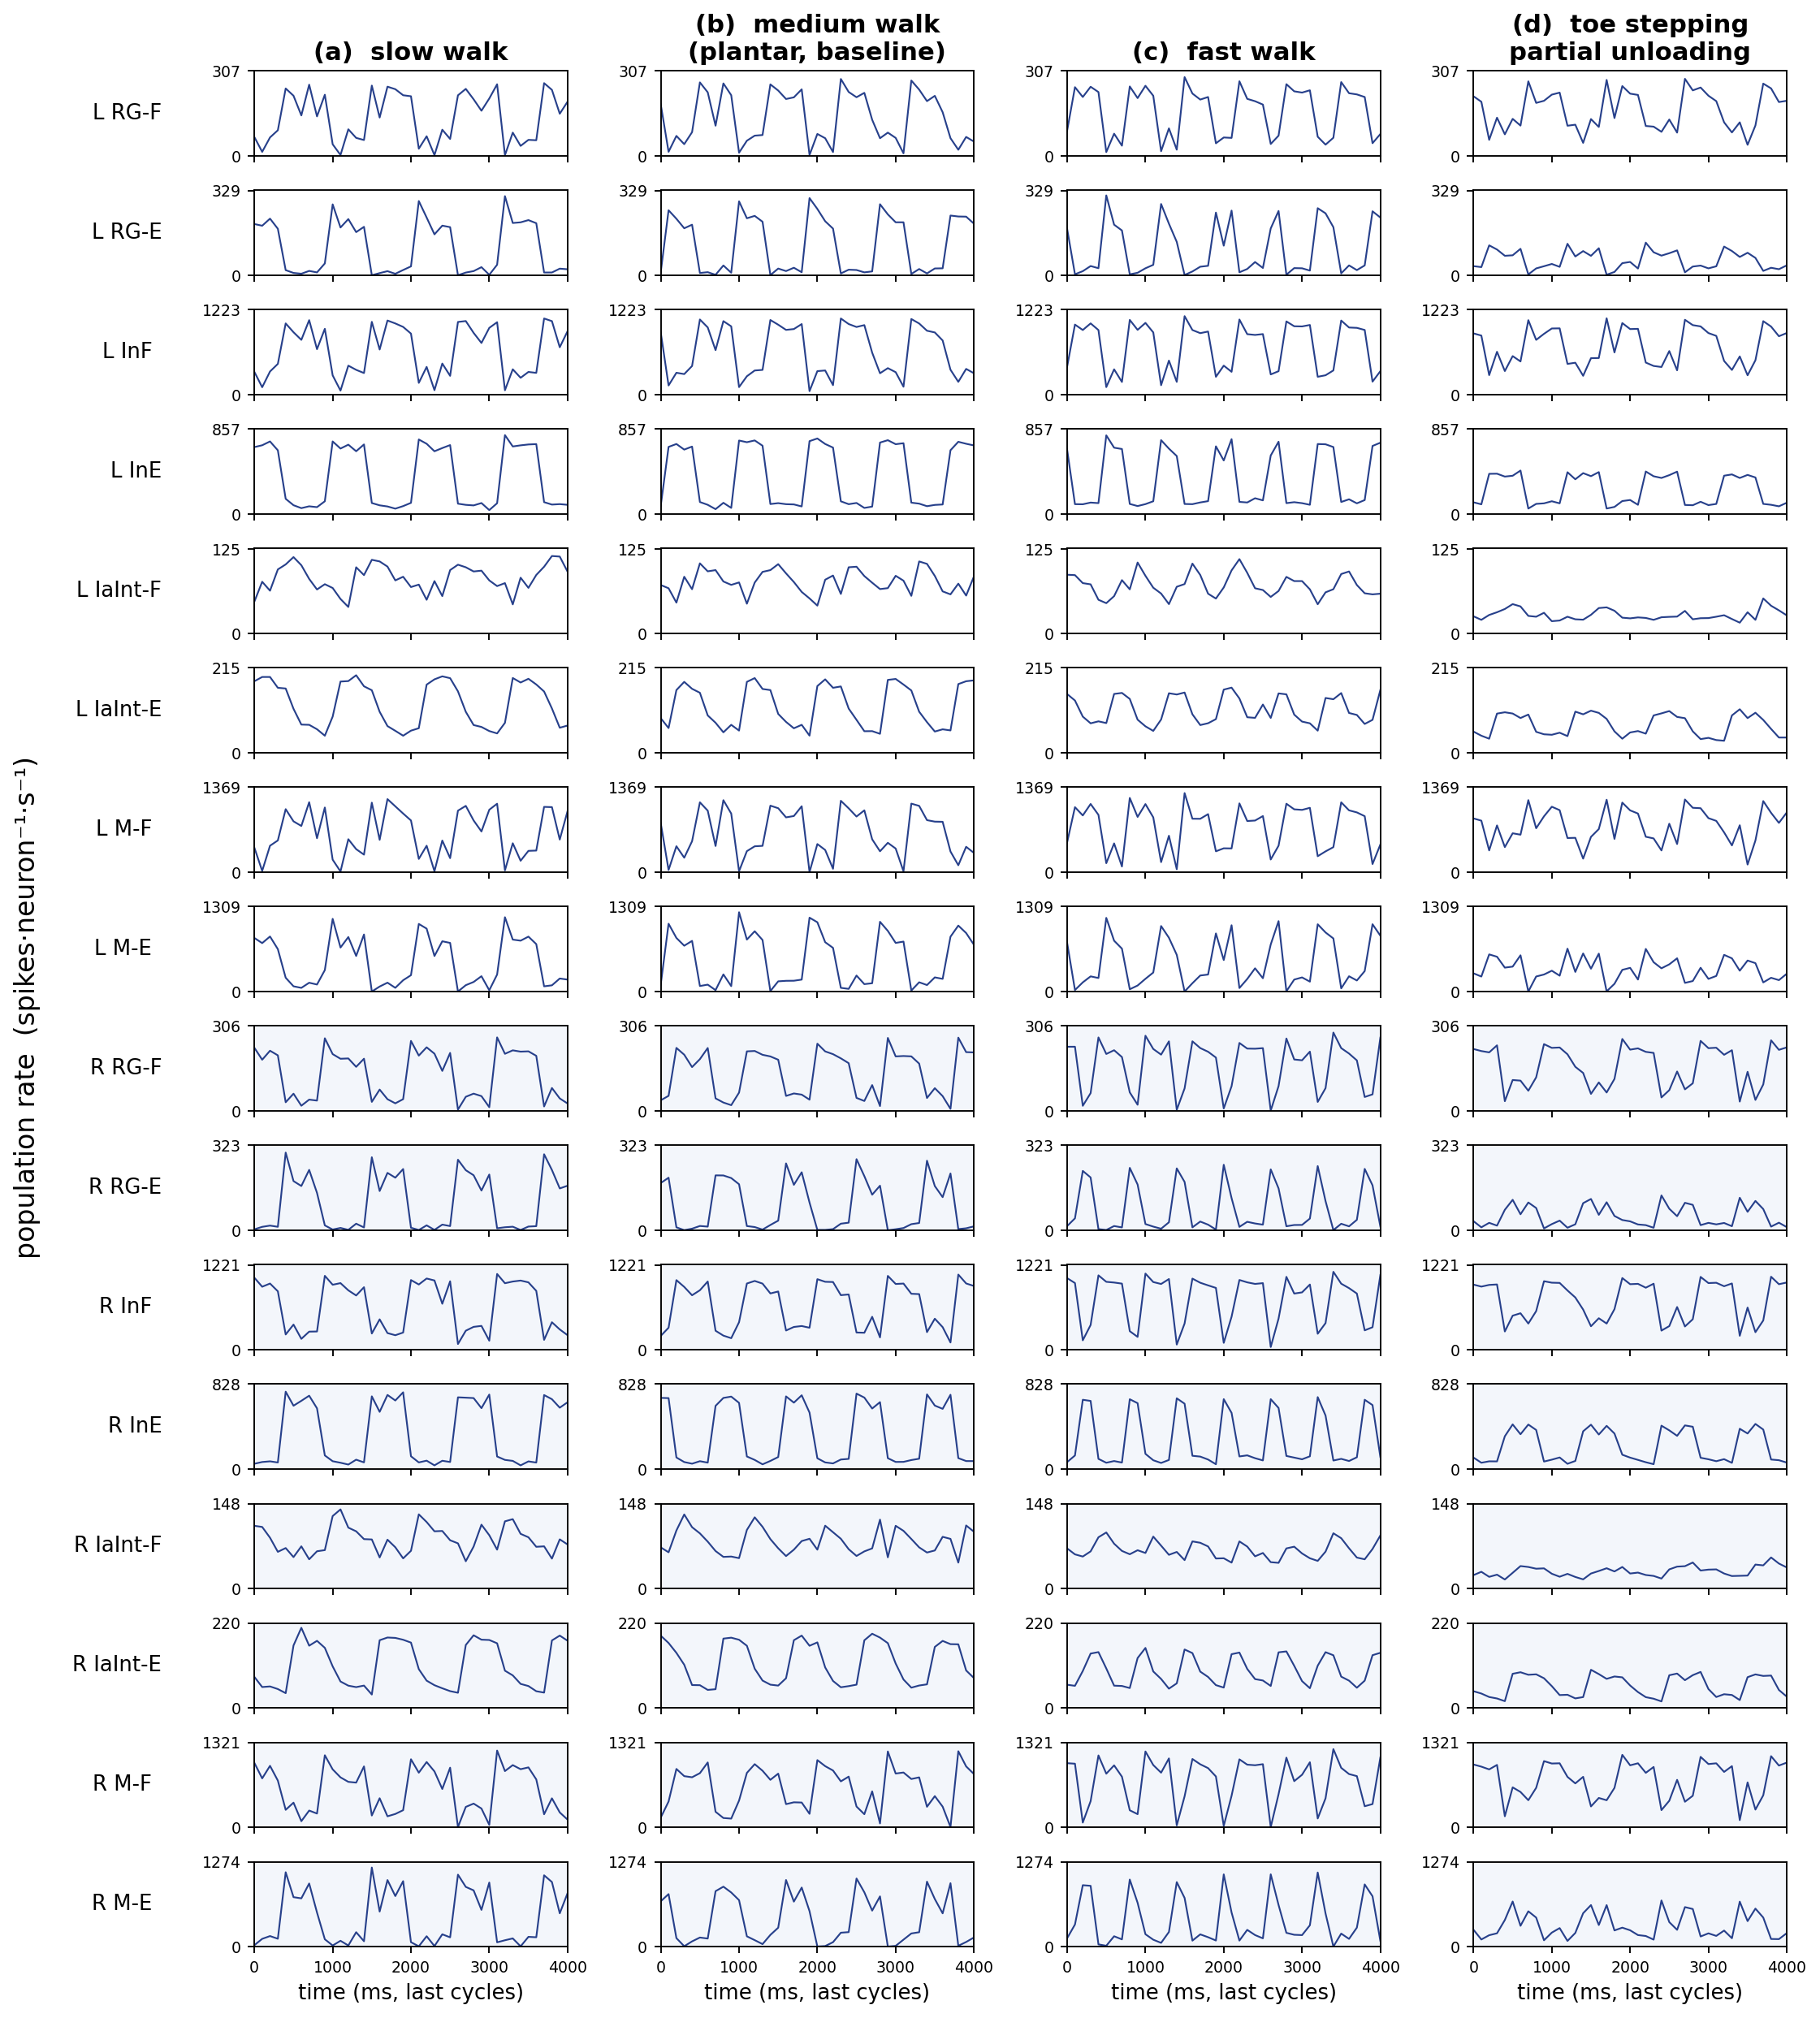
\includegraphics[width=0.95\textwidth]{fig_network_matrix_lam1em5.png}
  \caption{\textbf{Full-circuit population activity, $\lambda=10^{-5}$.} Same
    layout as Figure~\ref{fig:net_l2}. With the cutaneous weight still
    developing, left--right alternation is weaker, most visibly in fast walk
    and toe stepping.}
  \label{fig:net_l5}
\end{figure}

\begin{figure}[t]
  \centering
  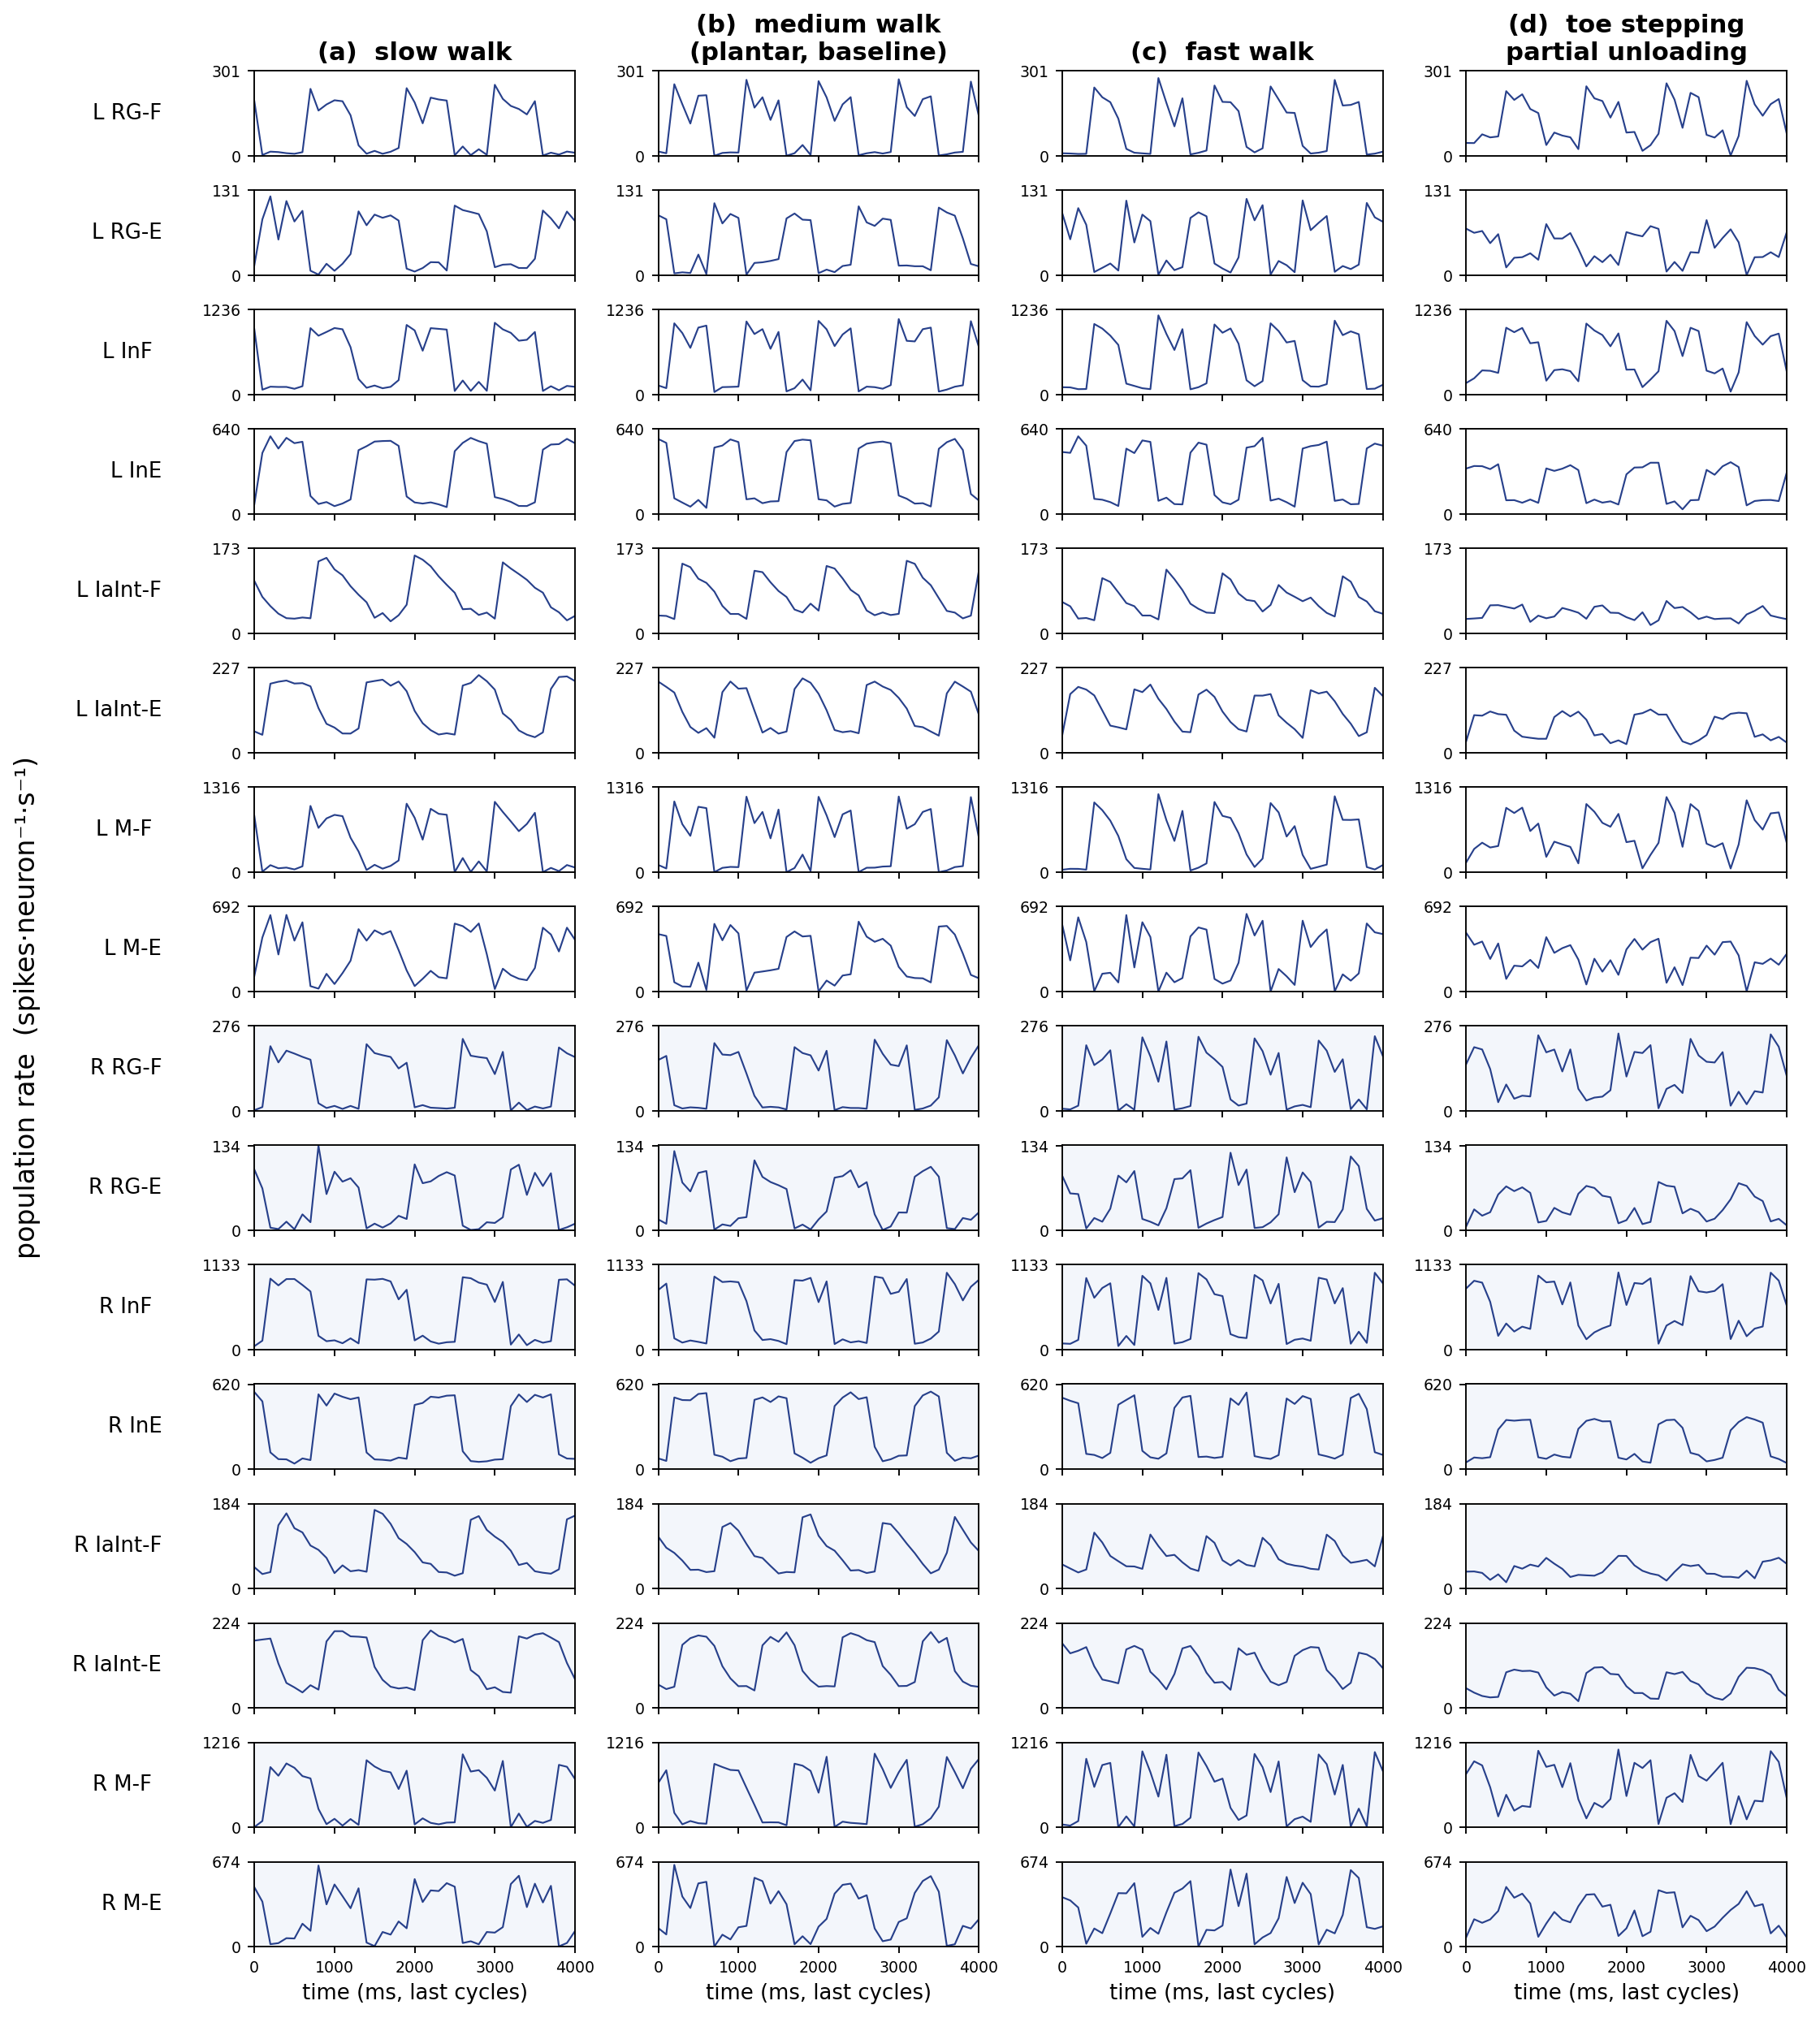
\includegraphics[width=0.95\textwidth]{fig_network_matrix_lam1em6.png}
  \caption{\textbf{Full-circuit population activity, $\lambda=10^{-6}$
    (slowest rate).} Same layout as Figure~\ref{fig:net_l2}; stance timing is
    set mostly by the timeouts at this rate.}
  \label{fig:net_l6}
\end{figure}

% =============================================================
\subsection{Comparison across the 4 locomotion modes $\times$ 5 STDP rates}\label{sec:results:comparison}

To compare all twenty conditions at a glance, Figures~\ref{fig:mode_lambda_heat}
and~\ref{fig:mode_lambda_trend} and Table~\ref{tab:mode_lambda} reduce each
condition to six numbers measured over the last $20$\,s: extensor/flexor
alternation of the forces [corr$(F_E,F_F)$] and of the rhythm generators
[corr(RG-E,RG-F)], left--right alternation [corr$(F_{E,L},F_{E,R})$], the
fraction of stance bouts ended by the timeout, peak extensor force, and the
learned CUT$\to$RG-E weight. Three patterns stand out.

\textbf{(i) Learning is what turns the loop on.} From $\lambda=10^{-2}$ to
$10^{-4}$ stance essentially always ends on the force threshold (no stance bout
at the timeout over the last 20\,s; at most $7\%$ on one leg from $t=30$\,s),
and the legs alternate (corr$(F_{E,L},F_{E,R})$ $-0.55$ to $-0.81$, except fast
walk at $10^{-2}$, $-0.32$). At $10^{-6}$, where the synapses do not learn, the timeouts take over
in every mode ($41$--$95\%$ of stance bouts), and at $10^{-5}$ in toe stepping
($100\%$). A closed, force-triggered gait therefore requires a learned
cutaneous synapse; without one the network falls back on its safety timer.

\textbf{(ii) The worst gait is at a partially learned weight.} At
$\lambda=10^{-5}$, with CUT$\to$RG-E at $\approx7$--$14$\,pA, the loop is
closed in the walking modes but poorly coordinated: extensor/flexor alternation
is the weakest of the grid (corr$(F_E,F_F)$ $-0.18$ to $-0.49$) and left--right
alternation drops in medium and fast walk and in toe stepping. A partially
developed cutaneous drive is strong enough to take over the timing of stance but
not strong or well-timed enough to organise it; with no learning at all the
timer is more regular, and with converged learning the sensory loop is.

\textbf{(iii) Speed and unloading.} Among the converged conditions, alternation
is best in slow and medium walk and falls in fast walk, where stance lasts only
$\approx190$\,ms. Partial unloading lowers extensor/flexor alternation
moderately and slows learning, but toe stepping still produces a genuine,
alternating gait once the cutaneous weight has converged. The rhythm generators
alternate strongly in every condition (corr(RG-E,RG-F) $\le-0.82$), including
those where the muscle forces do not: the counter-phase is lost at the muscle
level before it is lost at the rhythm-generator level.

\begin{figure}[t]
  \centering
  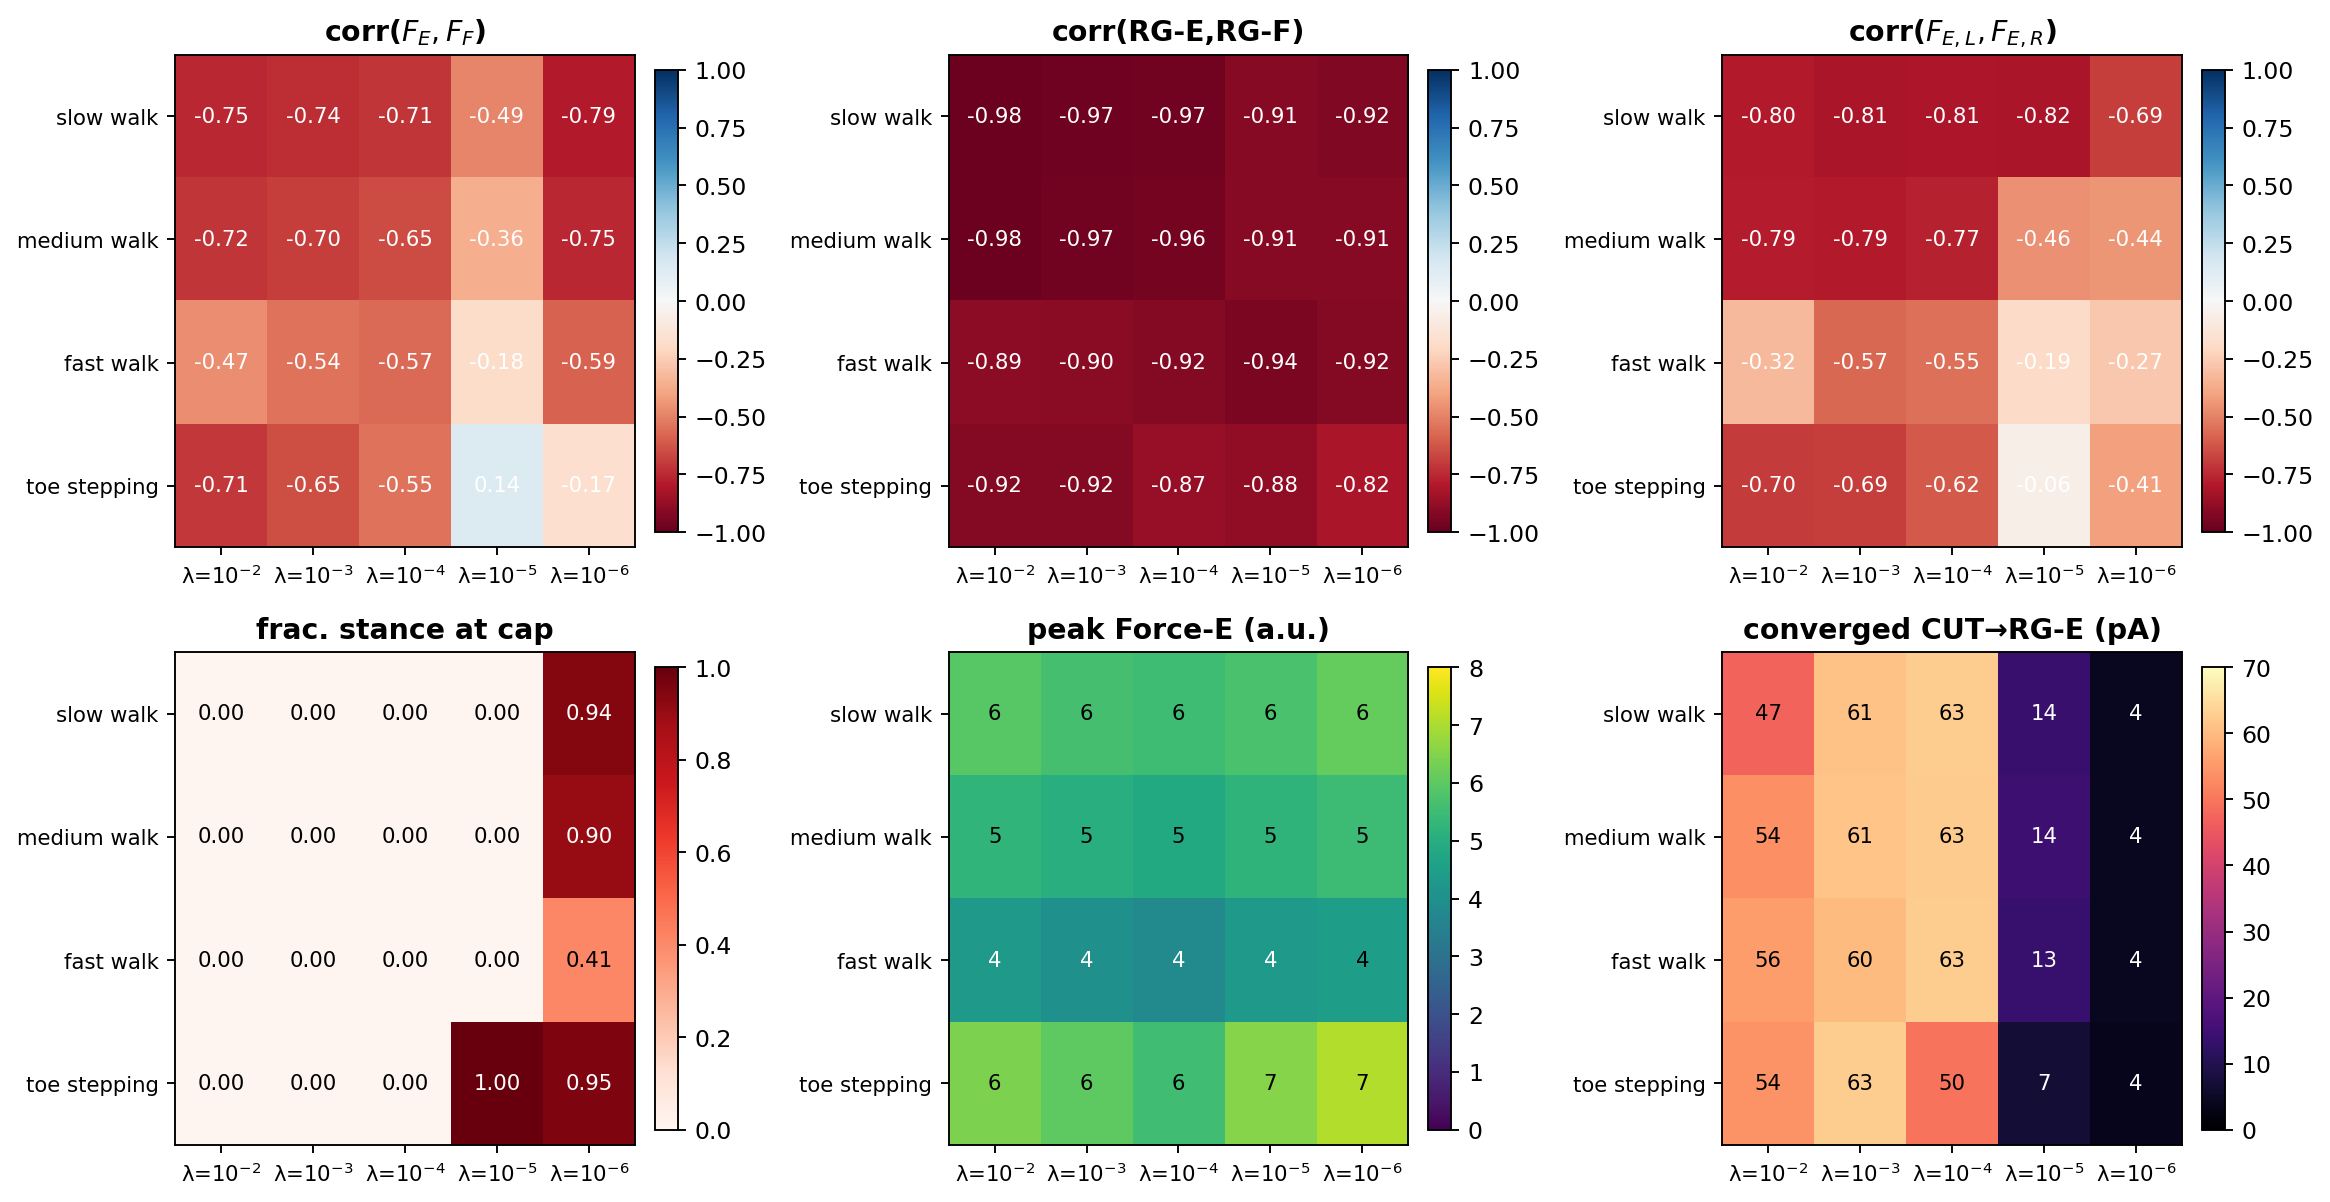
\includegraphics[width=0.95\textwidth]{fig_mode_lambda_heatmaps.png}
  \caption{\textbf{Metric heatmaps across the $4\times5$ grid} (rows: locomotion
    modes; columns: STDP rate $\lambda$). corr$(F_E,F_F)$, corr(RG-E,RG-F) and
    corr$(F_{E,L},F_{E,R})$ (diverging scale), fraction of stance bouts ended by
    the timeout (worst leg), peak Force-E (a.u.), and learned CUT$\to$RG-E weight
    (pA). Last 20\,s of each run; leg L unless stated.}
  \label{fig:mode_lambda_heat}
\end{figure}

\begin{figure}[t]
  \centering
  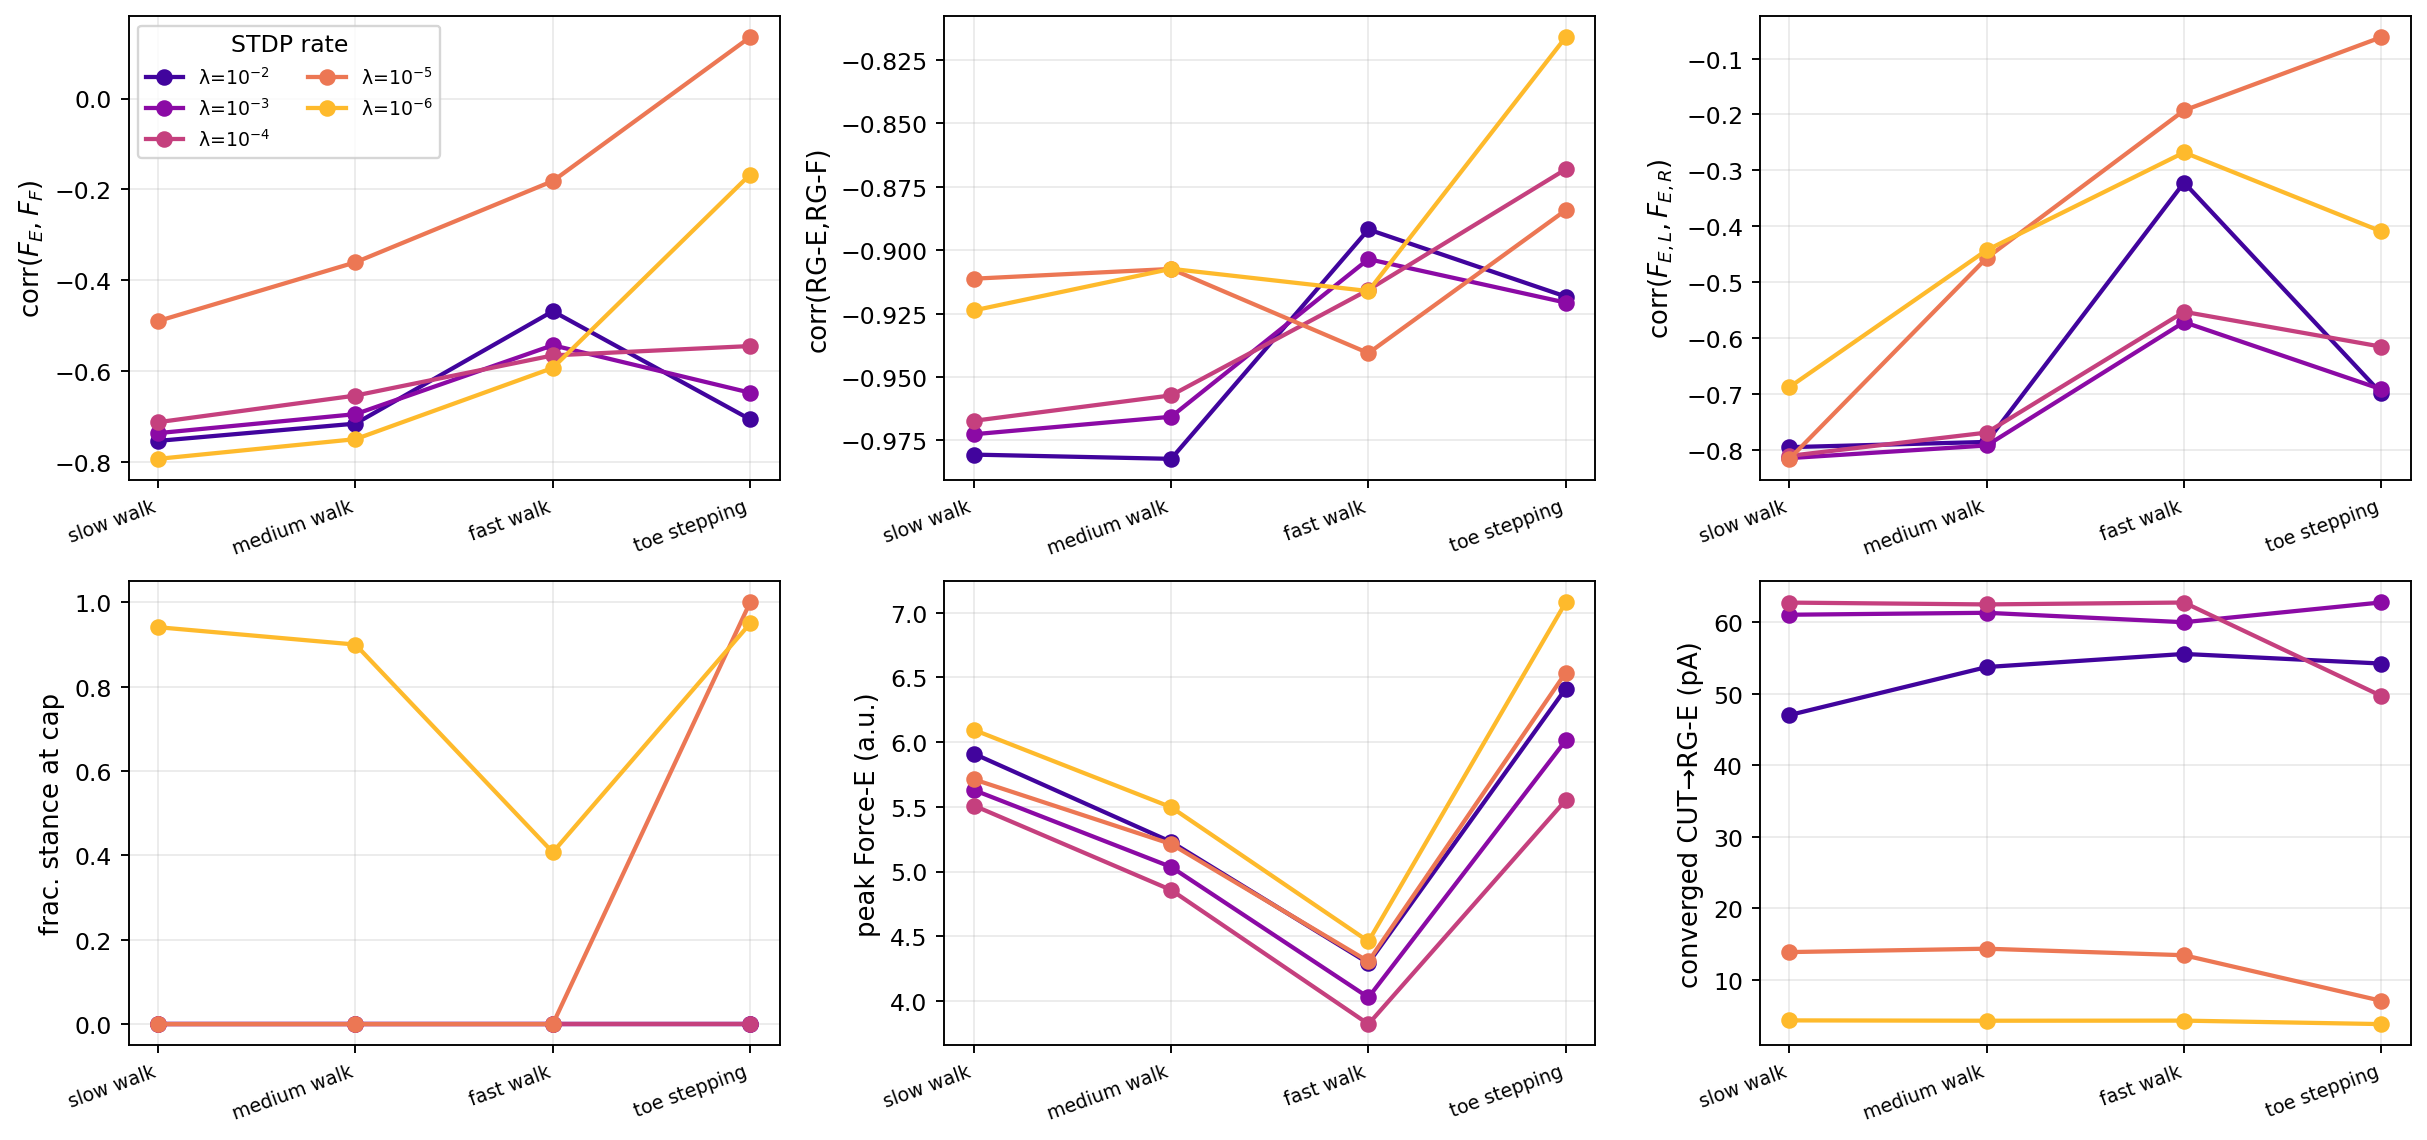
\includegraphics[width=0.9\textwidth]{fig_mode_lambda_trends.png}
  \caption{\textbf{Metric trends across the locomotion modes, one line per STDP
    rate $\lambda$.} Same six metrics as Figure~\ref{fig:mode_lambda_heat},
    plotted against the locomotion mode (slow walk $\to$ toe stepping).}
  \label{fig:mode_lambda_trend}
\end{figure}

\input{mode_lambda_table}


\section{Discussion}\label{sec:discussion}
\subsection{Summary of contributions}
We extended a computational sCPG model --- a two-legged half-centre
network in the Hodgkin--Huxley lineage
running from Rybak 2006 through Shevtsova 2015 and Danner 2017 to
Zhang 2022~\cite{rybak2006,shevtsova2015,danner2017,zhang2022} --- with four
mechanisms absent from that lineage: (i)
STDP that lets the network tune its own
cutaneous and descending synapses onto the rhythm generators rather than have
them hand-set; (ii) a closed loop from muscle-force feedback (Ia) into the
reciprocal-inhibition core; (iii) motoneuron pools driving explicit muscle
proxies with force, length and fatigue dynamics; and (iv) closed-loop stance
termination, in which each leg's stance ends when its own extensor force falls
rather than on a clock. Using this model we asked how a spinal
CPG's own synaptic weights should be organised to produce a stable walking
rhythm, and how that self-tuned rhythm depends on walking speed, on partial
unloading and on how fast the synapses can learn --- the variables manipulated
in rodent and human studies of SCI rehabilitation.

Three findings anchor the paper. First, the three plastic synapses --- the
cutaneous CUT$\to$RG-E projection and the brainstem BS$\to$RG-E and
BS$\to$RG-F projections --- converge to the same strength regardless of where
they start (from silent to $16$\,pA; \autoref{sec:results:robustness}), of
which leg they are in, and of walking speed or partial unloading
(\autoref{sec:results:weights}); the network organises its own gains rather
than requiring them to be prescribed by the modeller. Second, learning is what
closes the sensorimotor loop: once the cutaneous synapse has learned, stance is
ended by the leg's own force in every locomotion mode, whereas without learning
the network falls back on its safety timer (\autoref{sec:results:comparison}).
Third, the worst gait is produced not by the absence of learning but by a
partially learned synapse, strong enough to take over the timing of stance but
too weak to organise it (\autoref{sec:results:comparison}).

\subsection{Relation to prior computational and experimental sCPG work}
Zhang et al.\ (2022)~\cite{zhang2022} name two limitations of their own
four-rhythm-generator computational sCPG model explicitly: it has no
biomechanics or sensory feedback, and it has no motoneurons, treating
rhythm-generator output as a direct stand-in for motor output. Every
synaptic weight in their model, like its Rybak/Shevtsova/Danner
predecessors, is hand-tuned. Our model addresses both limitations for a
single hindlimb pair: the Ia force/length feedback loop supplies the
missing sensory closed loop, and explicit motoneuron pools driving a
saturating muscle model supply the missing motor periphery. On top of this
we add a mechanism none of these models have --- activity-dependent
plasticity on the afferent synapses --- so that the descending and
cutaneous gains are discovered by the network rather than fixed by the
experimenter.

The trade-off is architectural detail. Zhang et al.\ resolve genetically
identified commissural and long-propriospinal interneuron classes (V0V,
V0D, V1, V2a, V3, Shox2) across four limbs and reproduce V3-silencing
experiments quantitatively; our model collapses the commissural pathway to
two hand-set inhibitory projections between homologous half-centres and
covers only one limb pair. We also do not reproduce gait-transition
phenomena (walk $\to$ trot $\to$ gallop $\to$ bound): our stance timing is
closed-loop, but walking speed is set by per-mode fatigue and timeout constants
rather than emerging from a single tonic-drive parameter.
The two efforts are complementary rather than competing: theirs
demonstrates architectural realism at the cost of a closed loop; ours
demonstrates a closed, self-organising loop at the cost of architectural
detail. A natural synthesis --- hand-curated interlimb architecture wrapped
in a plastic, closed sensorimotor loop --- is a direct extension of both.

Our loading manipulation is drawn from a second, experimental lineage: the
rat and human spinal-cord-injury work of Courtine, Lavrov, Edgerton,
Gerasimenko and colleagues, in which stepping is studied across a graded
series of load-bearing conditions, from fully weight-supported walking to
hindlimb suspension~\cite{lavrov2008,edgerton2008,courtine2009,harkema2011}.
That literature establishes, largely from kinematic and electromyographic
readouts, that load-related afferent input shapes spinal stepping. Our model
offers a mechanistic, spiking-network account of one part of that picture: the
paw-contact signal both triggers the stance/swing transitions and trains the
synapse that makes those transitions reliable, so partial unloading weakens
the gait and slows its acquisition (\autoref{sec:results:weights},
\autoref{sec:results:comparison}). In that sense the model is positioned to
connect the computational sCPG lineage above with this experimental
SCI-rehabilitation lineage, and we return to that connection in the Clinical
implications below.

\subsection{A partially learned synapse is worse than none}
One finding deserves a mechanistic reading before its clinical one. The gait
is worst at $\lambda=10^{-5}$, where the cutaneous synapse has grown to only
$\approx7$--$14$\,pA by the end of the run, not at $\lambda=10^{-6}$, where it
has not grown at all (\autoref{sec:results:comparison}). With no learning the
extensor force rarely reaches the stance-termination threshold, so stance
bouts run to the timeout and the timeouts impose a regular, clock-like
alternation. With converged learning the cutaneous drive produces a strong,
well-timed extensor burst and the force threshold ends each stance reliably.
In between, the drive is strong enough that the force threshold, rather than
the timer, decides when stance ends, but too weak to make that decision
consistent from step to step, so both extensor/flexor and left--right
coordination degrade. The same logic applies along the loading axis: at
$\lambda=10^{-5}$ toe stepping, with half the cutaneous drive, has not even
reached that intermediate regime and still runs on the timer. In both cases
\emph{some} correctly organised plastic drive is better than none, but a
partially organised one can be worse than either extreme.

\subsection{Clinical implications}
The present computational approach yields several insights for the
clinical rehabilitation of individuals with SCI. Apart from recapitulating
locomotor behaviour, the proposed computational framework provides a
mechanistic account of how sensorimotor interactions and activity-dependent
plasticity might enable functional recovery. First, sensory inputs are
critical for facilitating locomotor rehabilitation, not as a replacement
for lost supraspinal descending input, but as a catalyst for plastic
adaptation in the spinal cord sensorimotor networks.

Our simulation results show that, when appropriately controlled through
load and/or activity, such sensorimotor input drives spinal adaptation and
subsequently restores coordinated locomotor outputs
(\autoref{sec:results:weights}).

Weight-bearing conditions drove the cutaneous synapse to its plateau
quickly and stabilised locomotor output, whereas reduced support slowed that
learning and led to a less coordinated gait
(\autoref{sec:results:weights}, \autoref{sec:results:comparison}). These findings parallel clinical
observations that repetitive task-specific locomotor rehabilitation ---
body-weight-support treadmill walking, robot- and manually-assisted
stepping --- restores stepping in individuals with motor-incomplete SCI by
engaging residual plasticity in the spinal sensorimotor circuitry rather
than by regenerating damaged descending
pathways~\cite{wernigMuller1992,dietz1998,behrmanHarkema2000}.

\paragraph{Which injury this model corresponds to.}
The brainstem-to-rhythm-generator (BS$\to$RG) drive stays tonic and non-zero
throughout, so the model structurally represents a state in which some
supraspinal descending input survives the lesion --- clinically,
motor-incomplete SCI (ASIA Impairment Scale grades C/D), the population in
which BWSTT and robot- or manually-assisted training reliably restore
stepping~\cite{wernigMuller1992,dietz1998,behrmanHarkema2000}. Two kinds of
synapse are plastic, and they map onto different mechanisms. CUT$\to$RG-E is
intraspinal and caudal to the lesion; its strengthening models
activity-dependent reinforcement of an intact, underused sensorimotor loop ---
the mechanism BWSTT and related therapies are thought to exploit. BS$\to$RG is
the model's spared descending projection; its strengthening is the analogue of
the reorganisation of spared reticulospinal input that accompanies spontaneous
locomotor recovery after incomplete SCI in rats~\cite{ballermannFouad2006}.
Neither models repair of a severed pathway.

An additional clinically relevant observation is that the effectiveness of
recovery depends on the degree of plasticity. In the simulations, too little plasticity leaves the gait on its safety timer
and an intermediate, still-developing level of plasticity produces the least
coordinated gait of all (\autoref{sec:results:comparison}); the fastest rate
converges within seconds but leaves the learned weights fluctuating from step
to step below their plateau, with weaker left--right alternation in fast walk.
The useful range of plasticity would thus correspond to rates that let spinal
motor networks complete their adaptation within the training period while
avoiding step-to-step instability, a heuristic that may help in choosing
rehabilitation intensities and in managing the effects of pharmacological or
electrical neuromodulation therapies on spinal adaptation.

\paragraph{Interpreting the learning-rate axis as plasticity capacity.}
One natural reading of the $\lambda$ axis is developmental. The capacity
for activity-dependent synaptic change is not fixed across the lifespan:
it is greatest during early postnatal critical periods and declines with
maturity, and correspondingly, neonatal and juvenile rodents recover
locomotor function after spinal injury considerably better than adults.
It is therefore tempting to read our fastest learning rates as
``younger'' and our slowest as ``older'' animals.\todo{cite developmental
critical-period / age-related decline in spinal plasticity and
age-dependent locomotor recovery after SCI} We suggest this analogy
should be treated as a qualitative ordering rather than a calibration:
$\lambda$ is a phenomenological STDP rate constant, it was not fitted to
any measurement of plasticity in animals of a given age, and age is only
one of several determinants of plasticity capacity --- time since injury,
prior activity history, and pharmacological or electrical neuromodulation
all modulate the same underlying quantity. Read this way, the $\lambda$
axis is better described as spanning \emph{plasticity capacity}, of which
age is one contributor.

With that caveat, the interpretation yields a concrete and testable
prediction. Because gait quality in our sweep does not increase
monotonically with $\lambda$ --- it is worst at an intermediate, incompletely
converged rate, and at the fastest rate the learned weights stay unstable
(\autoref{sec:results:comparison}) --- the model predicts that recovery
depends on plasticity being sufficient to \emph{complete} adaptation within
the training period, and that more plasticity is not automatically better. This resonates with the clinical picture in
which excessive or misdirected plasticity after SCI manifests as
maladaptive outcomes such as spasticity, aberrant sprouting and
neuropathic pain rather than improved locomotion.\todo{cite maladaptive
plasticity after SCI} The prediction is directly testable by running the
same rehabilitation protocol across age groups and asking whether
intermediate-age animals show the best coordination recovery, which would
be a stronger validation of the learning-rate axis than any of the
comparisons we are currently able to make.

Furthermore, the present computational framework might serve as a useful
tool for designing, optimising, and validating interventions before their
clinical application.

It is feasible to investigate, via simulation studies, various clinical
rehabilitation interventions (e.g., robot-assisted walking at various
assistance levels and weight-supported environments, ESCS at different
locations and frequencies, combination therapies) to identify the most
effective, non-invasive treatments. Finally, integrating this framework
with individual patient-specific data might pave the way for the
development of virtual-twin approaches that could predict, simulate, and
optimise patient outcomes after specific rehabilitation therapies in a
highly personalised fashion.

\subsection{Limitations}
In addition to the positive implications outlined above, it is important
to note some limitations of the proposed model. To simplify the biological
complexity of the spinal locomotor system, a level of abstraction was used
in defining sensorimotor pathways, interneurons and motor outputs. The
model does not include an adaptive supraspinal control mechanism (the
brainstem drive is a tonic input), detailed muscle-tendon
biomechanics beyond the saturating force/activation/fatigue model used here,
or longer-term structural plasticity.

It also omits features of SCI such as chronic damage to the dorsal and
ventral roots, glial scarring, or the diversity of human SCI.

It should also be highlighted that the model was not calibrated on any
experimental data collected from actual individuals with SCI. Hence the
values of the STDP parameters can only be viewed as computational
representations of plasticity rather than direct measures of spinal
learning capacity. Consequently, the present model should be interpreted
as hypothesis-generating rather than predictive in nature, and further
studies incorporating more detailed muscle dynamics, more realistic
sensory transduction, supraspinal inputs, and patient-specific data will
be required to establish greater biological realism.

These conceptual limitations are compounded by several specific modelling
choices worth stating explicitly:

\begin{enumerate}
  \item \textbf{Interneuron and interlimb detail.} We resolve two hand-set
        commissural projections rather than the genetically identified
        V0/V1/V2a/V3 interneuron classes, and we model one hindlimb pair
        rather than fore--hindlimb coordination~\cite{zhang2022}; we
        likewise do not reproduce gait-transition phenomena
        (walk $\to$ trot $\to$ gallop $\to$ bound).
  \item \textbf{Swing is timed, not sensed.} Only the end of stance is
        force-triggered; the model has no hip-position or other swing
        termination signal, so every swing lasts its timeout and
        stride-to-stride variability arises from stance alone.
  \item \textbf{Stride periods.} The measured strides ($\approx0.6$\,s fast
        walk to $\approx1.0$\,s slow walk) are long for a trotting rat,
        because every swing lasts its full timeout; locomotion modes are
        therefore defined by their operating points (Table~\ref{tab:modes}),
        not by treadmill speed.
  \item \textbf{Full unloading not reproduced.} At air-stepping loading the
        extensor force is too small for the force-triggered stance detector,
        so the loading axis stops at toe stepping.
  \item \textbf{Per-mode operating points.} Fatigue and timeout constants
        were chosen per mode, and a small persistent left--right fatigue
        asymmetry is needed at the fast and toe-stepping points to keep the
        legs from falling into in-phase stepping.
  \item \textbf{No stochastic replication.} Each condition is a single run
        and multi-threaded runs are not bit-reproducible; the ten-point
        initial-weight sweep (\autoref{sec:results:robustness}) substitutes
        for repeated stochastic trials in establishing that a result is not
        an artefact of a particular initialisation.
\end{enumerate}

\subsection{Concluding remark}
A computational sCPG half-centre oscillator, closed in the loop with
motoneurons, muscle proxies, and load-dependent sensory feedback that itself
decides when stance ends, tunes its own cutaneous and descending gains through
spike-timing-dependent plasticity to a stable set-point --- one that is
independent of how the network starts and of walking speed. Learning is what
turns the sensory loop on: without it the gait falls back on a safety timer,
and a partially learned synapse produces the least coordinated gait of all.
Partial unloading slows that learning and weakens the gait without abolishing
it. Beyond the specific findings, the model
demonstrates that a spinal CPG's descending and sensory gains need not be
prescribed by the modeller: given a plastic synapse, appropriately timed
sensory drive, and enough time, the network finds them on its own. That
property, together with the model's explicit and inspectable parameters,
is what makes it a plausible substrate for exploring --- and eventually,
with patient-specific calibration, for helping to design --- sensorimotor
rehabilitation strategies after spinal cord injury.


% --- Data, code, reproducibility ---
\section*{Code and data availability}
All source code is available at
\href{https://github.com/max-talanov/tinyCPG}{github.com/max-talanov/tinyCPG}.
Raw HDF5 simulation outputs underlying Figures~\ref{fig:main}--\ref{fig:speed}
are deposited at \todo{Zenodo DOI}.

\section*{Acknowledgements}
\todo{add funding, computational allocation MN5/BSC, collaborators.}

% --- Bibliography ---
\bibliographystyle{unsrt}   % switch to PLOS or Frontiers style at submission
\bibliography{refs}

\end{document}
